\subsection{Prototypical Networks}
\begin{table}[h!]
\centering

\begin{tabular}{|l|c|c|}
\hline
 & Support (\%) & Query (\%)\\
\hline
Train & 99.96 & 99.84\\
\hline
Validation & 99.72 & 99.39\\
\hline
\end{tabular}
\caption{Accuracies finales de ProtoNet sobre MNIST para support y query.}
\label{tab:proto accs}
\end{table}

En la tabla~\ref{tab:proto accs} se registran las accuracies conseguidas por ProtoNet. El alto rendimiento del support set se explica, en su mayor parte, por el hecho de que es el mismo conjunto sobre el que se calculan los prototipos. El resultado principal de la tabla es la accuracy casi igual conseguida por query, indicando que los prototipos construidos a partir de support logran generalizar correctamente a ejemplos no vistos dentro de cada tarea.

\begin{figure}[H]
    \centering
    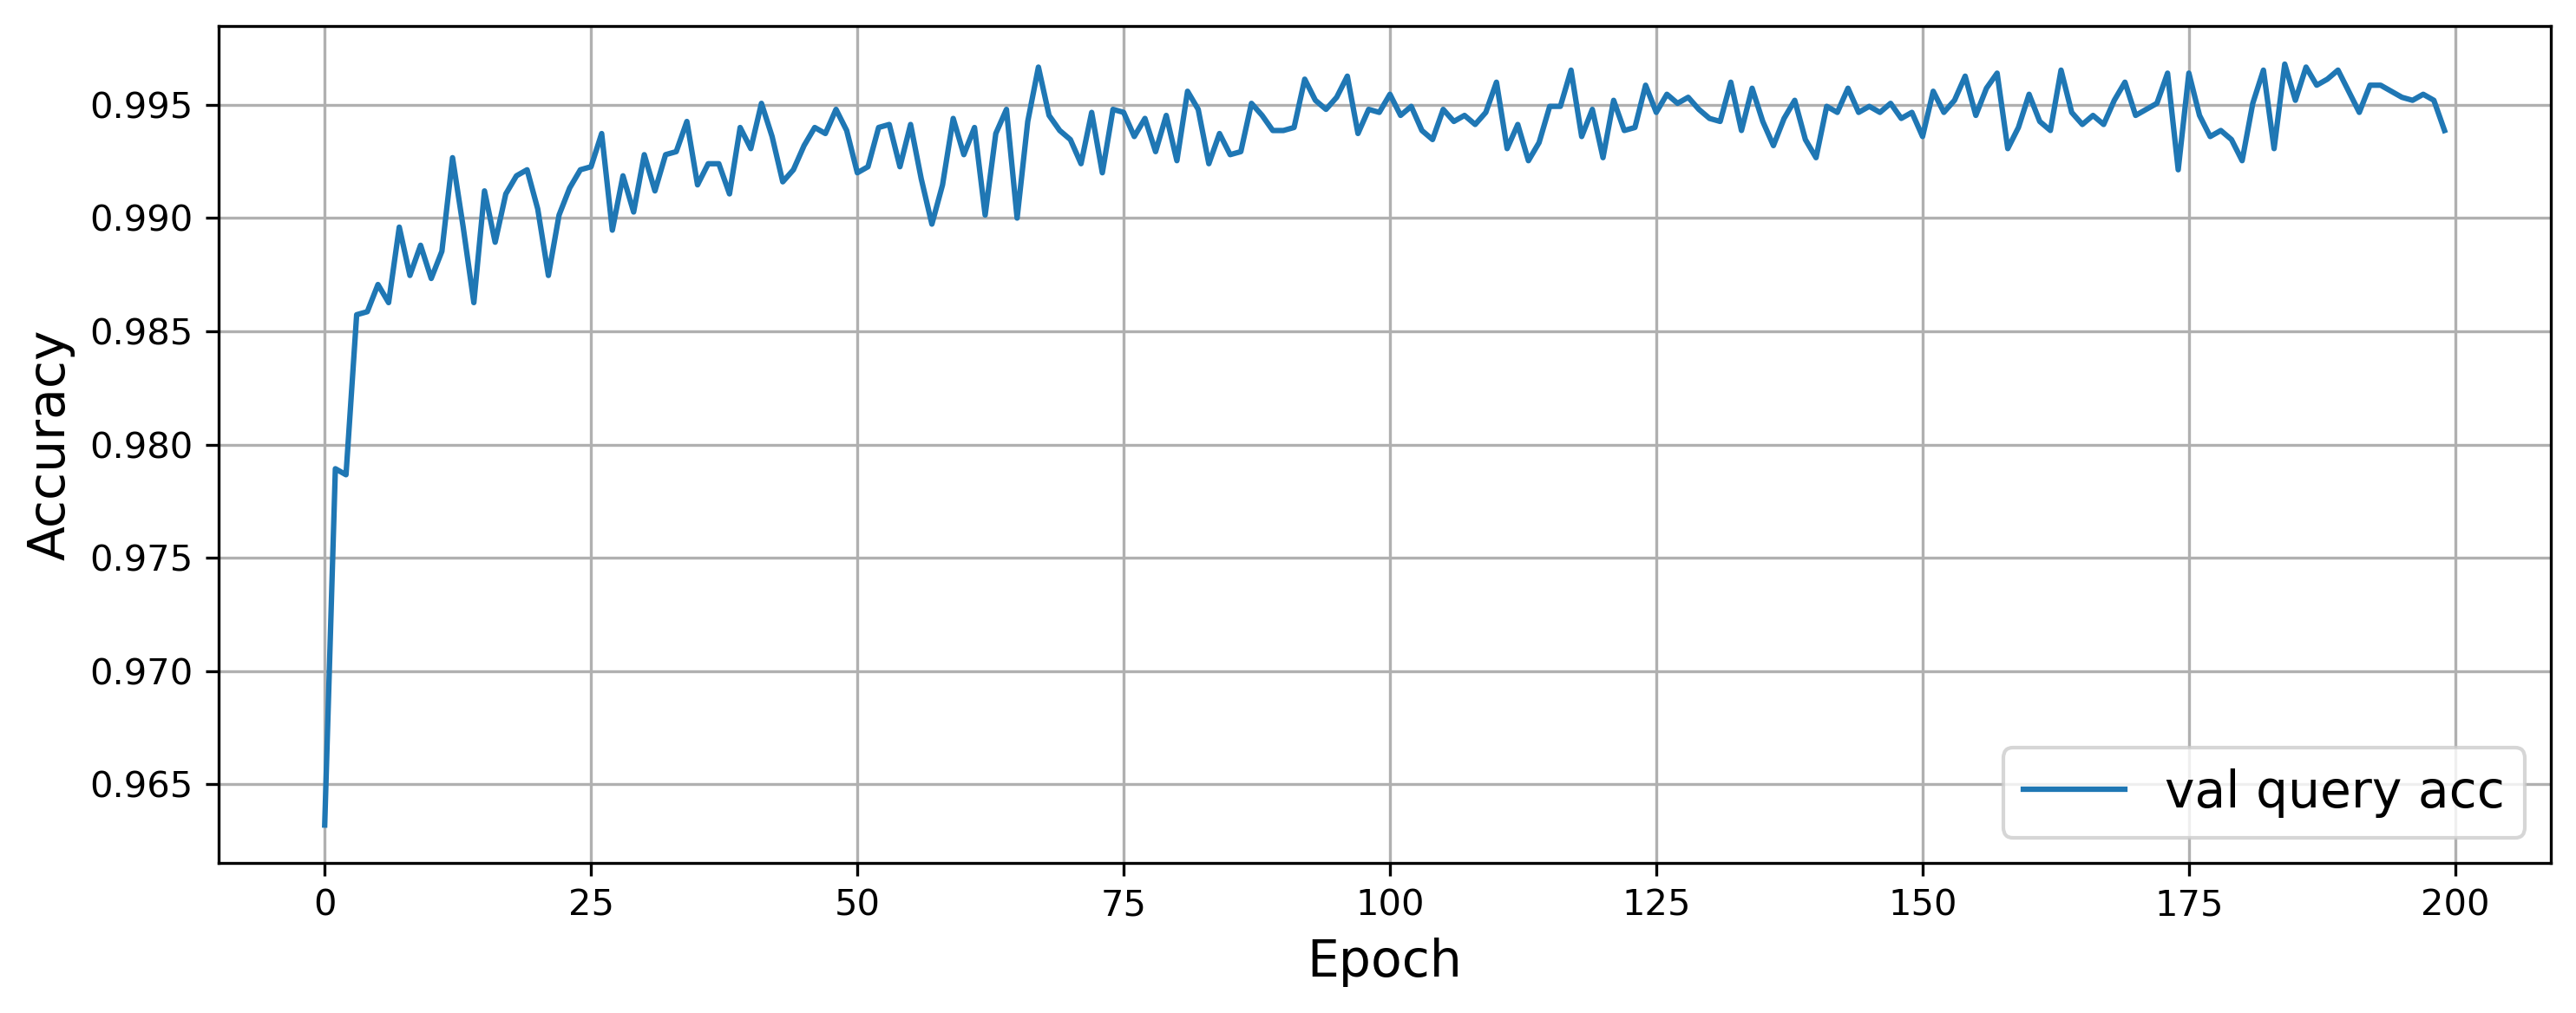
\includegraphics[width=0.8\textwidth]{../images/protonet/protonet_training.png}
    \caption{Accuracy de query en validación a lo largo del entrenamiento. }
    \label{fig:protonet training}
\end{figure}

% ¿Se forman clusters separados? ¿Cómo evoluciona la estructura a medida que avanza el entrenamiento?

En la figura~\ref{fig:protonet training} se muestra la evolución de la accuracy sobre el set de validación de query. Se observa un incremento rápido durante las primeras épocas y luego una oscilación en valores altos cercanos a 0.995. Esa oscilación surge del sampleo realizado durante el entrenamiento. 

\begin{figure}[H]
    \centering
    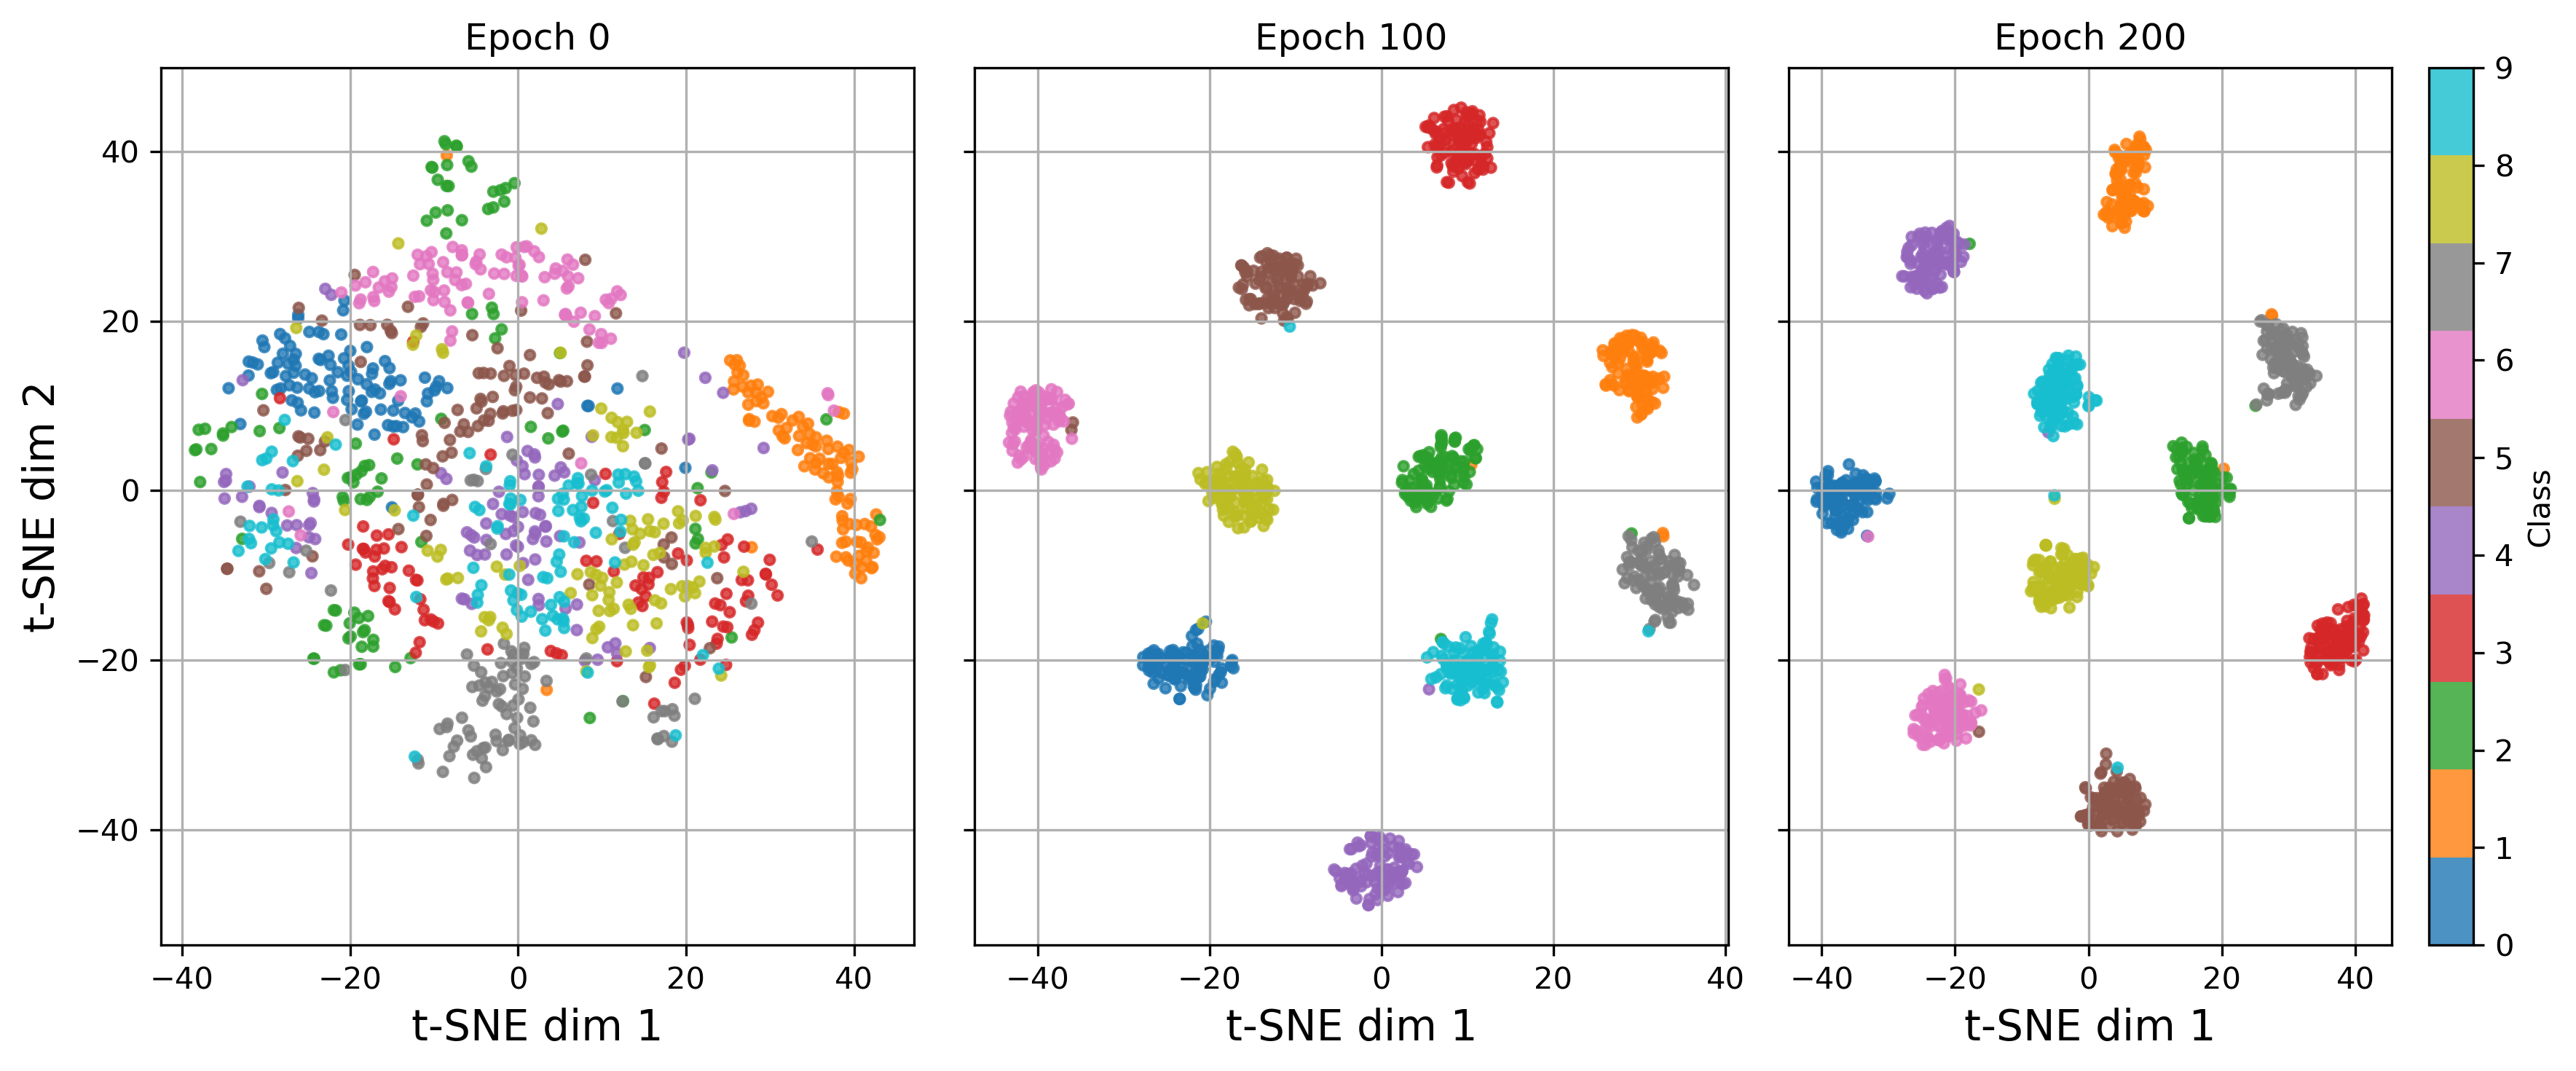
\includegraphics[width=0.8\textwidth]{../images/protonet/protonet_training_tsnes.png}
    \caption{t-SNE de los embeddings del encoder para un conjunto de imágenes de MNIST al inicio, a mitad y al final del entrenamiento.}
    \label{fig:protonet training tsnes}
\end{figure}

% ¿Se forman clusters separados? ¿Cómo evoluciona la estructura a medida que avanza el entrenamiento?

En la figura~\ref{fig:protonent training tsnes} se visualiza la evolución de los embeddings generados por el encoder sobre un conjunto de imágenes de MNIST. Antes del entrenamiento, las clases estan mayormente mezcladas y solo la clase 1 parece formar una especie de cluster con pocas muestras dispersas. En la época 100, en cambio, ya se distinguen clusters separados por clases, con pocas muestras mal distribuidas. Finalmente para la época 200 no se produce un cambio significativo.

\begin{figure}[H]
    \centering
    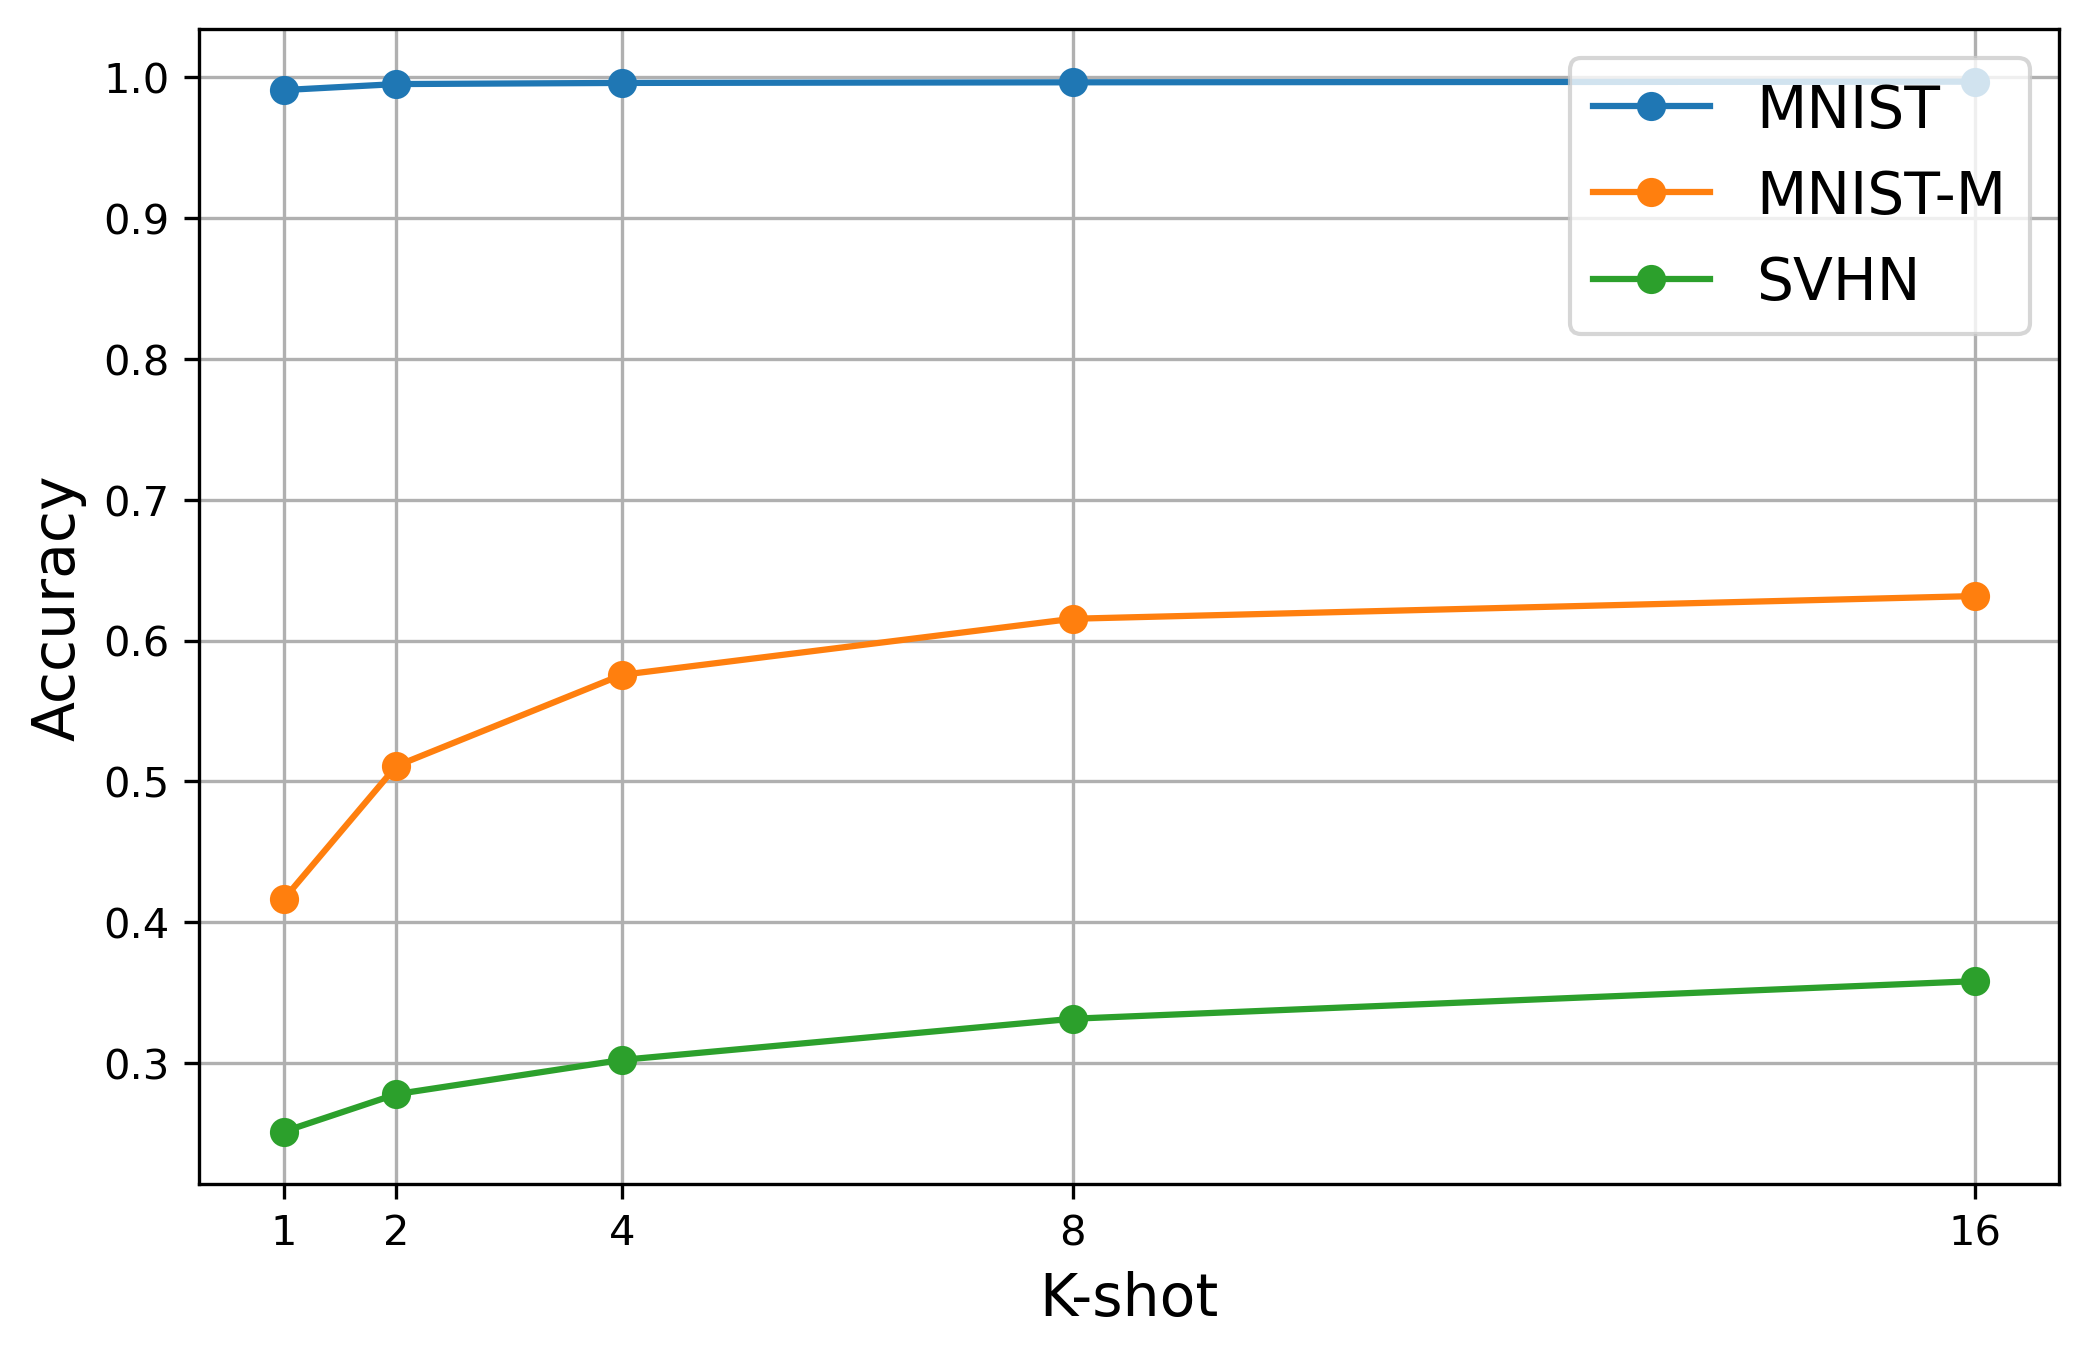
\includegraphics[width=0.6\textwidth]{../images/protonet/acc_vs_ks.png}
    \caption{Accuracy sobre el conjunto de test de MNIST con k = {1, 2, 4, 8, 16}.}
    \label{fig:protonet acc vs k}
\end{figure}

En la imagen~\ref{fig:protonet acc vs k} se evaluó el modelo sobre los conjuntos de testeo de todos los dominios para distintas $K$. 

En MNIST se observa una accuracy casi perfecta para todo $K$, dado que el modelo entrenó sobre esos datos y las figuras~\ref{fig:protonet training} y~\ref{fig:protonent training tsnes} demuestran que logra diferenciar y generalizar correctamente entre clases. Aumentar el valor de $K$ casi no modifica el desempeño ya que con una baja cantidad de ejemplos, los prototipos ya resultan lo suficientemente representativos.

En cambio, para los dominios MNIST-M y SVHN, la accuracy es considerablemente menor pero siempre creciente junto a $K$. También puede notarse que MNIST-M mantiene una accuracy de aproximadamente el doble de valor que SVHN para todos los valores de $K$. Esto puede explicarse por la similaridad entre MNIST y MNIST-M al ser el ultimo una modificación del primero, mientras que SVHN presenta un desplazamiento de dominio más fuerte.

También se considera necesario remarcar la forma de crecimiento de la accuracy junto a $K$. EN MNIST-M y SVHN, el aporte de cada muestra a la generación de prototipos es menor, indicando que no es necesario incluir todo el dataset para generar prototipos representativos.

\begin{figure}[H]
    \centering
    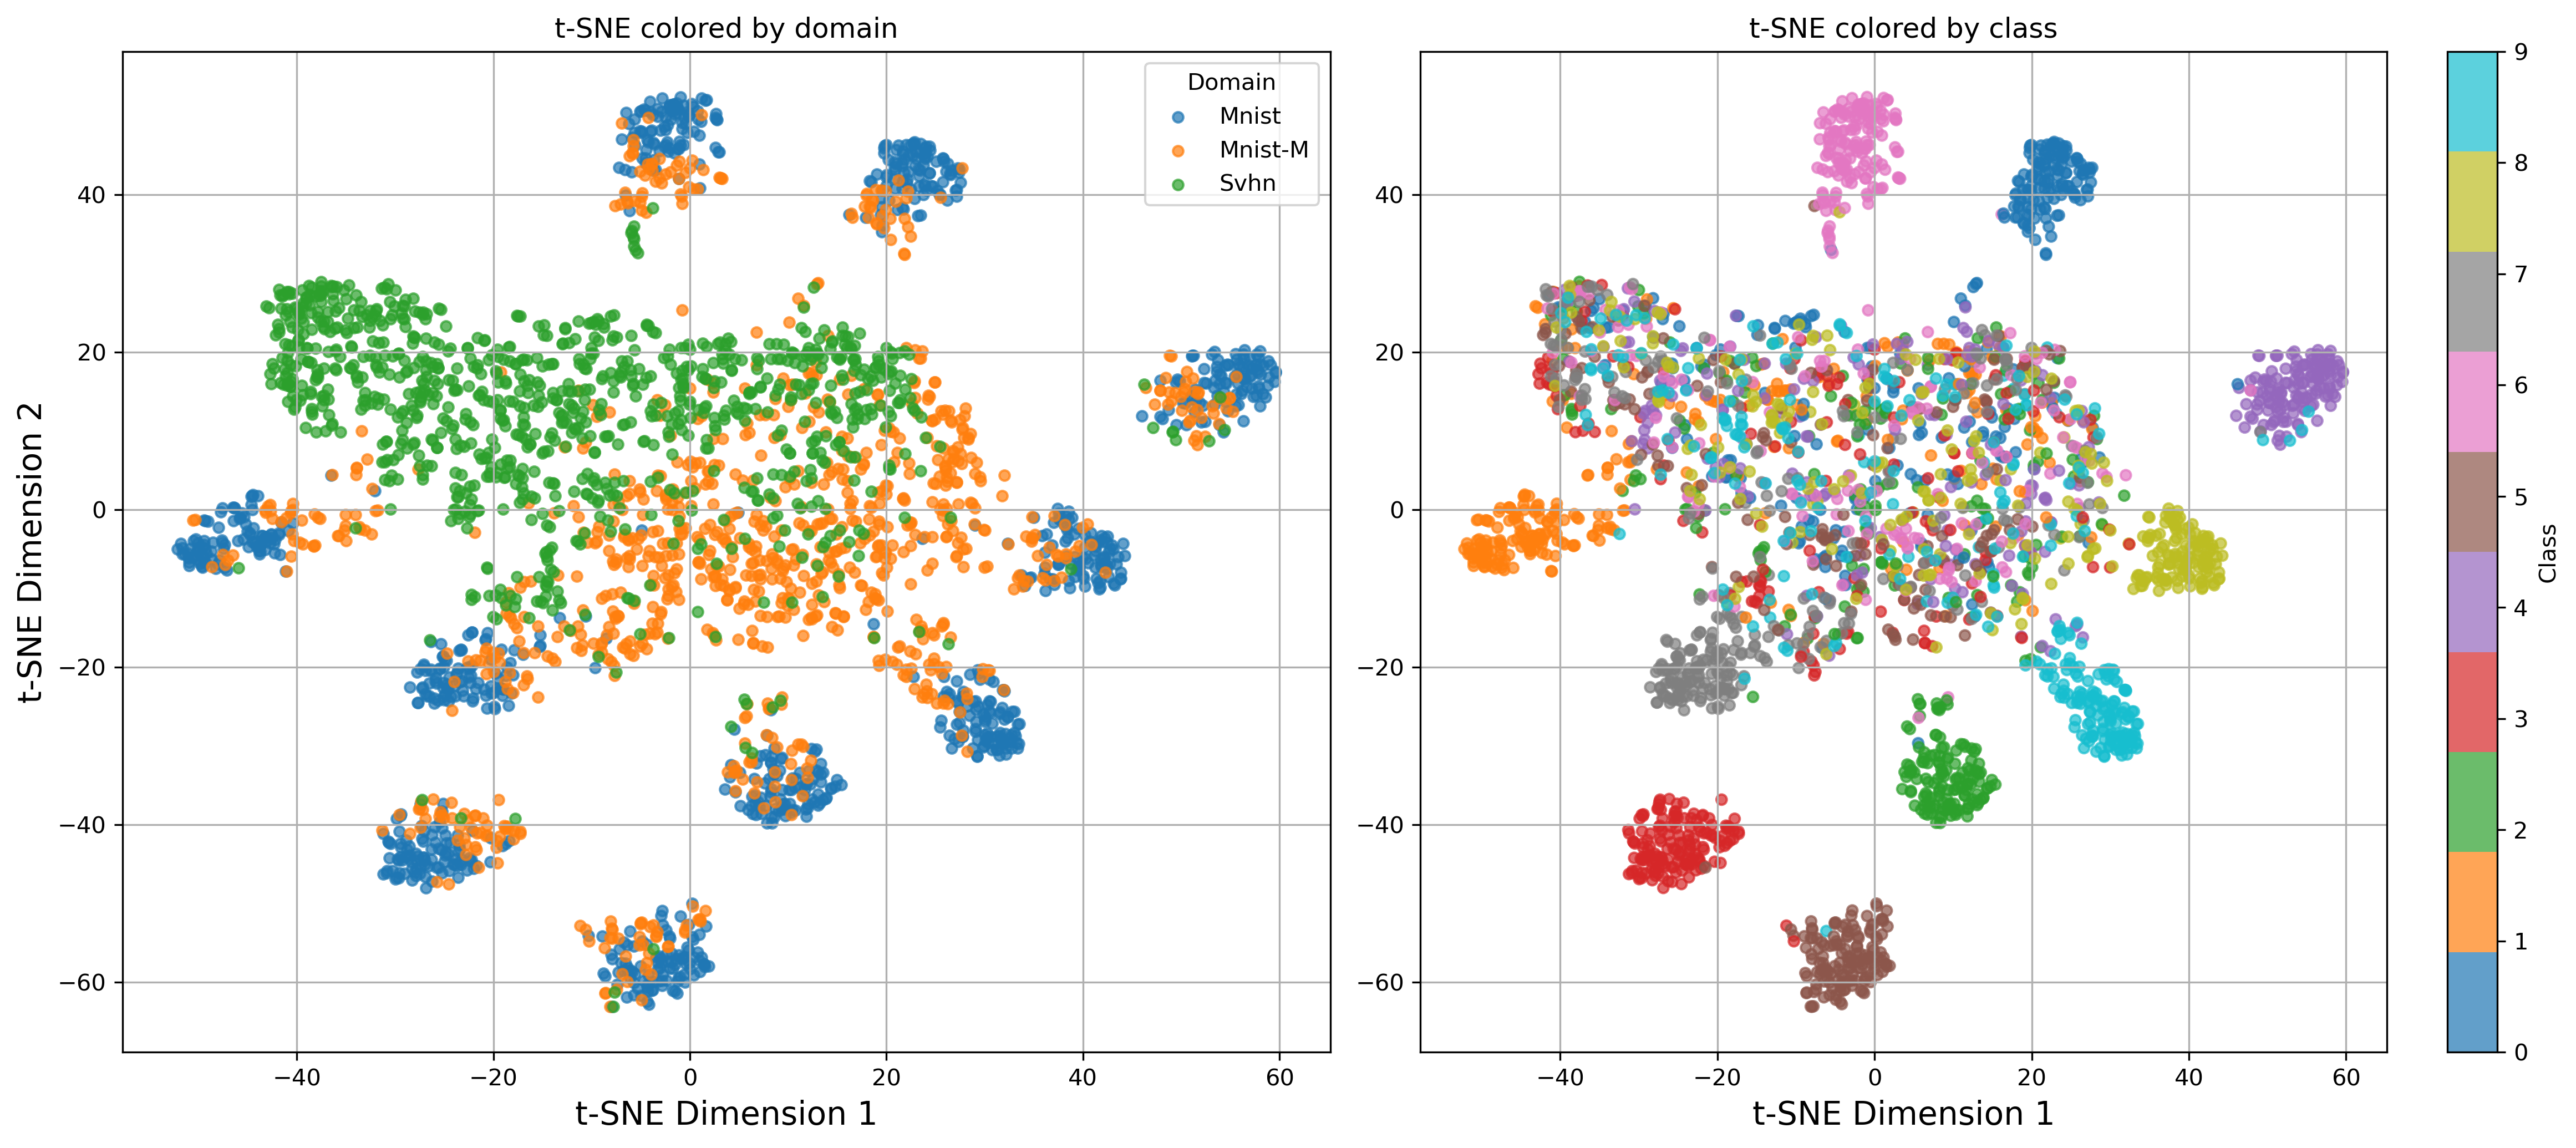
\includegraphics[width=0.8\textwidth]{../images/protonet/tsnes_domain_class.png}
    \caption{t-SNE de los embeddings del encoder para un conjunto de imágenes de prueba sobre los tres dominios.}
    \label{fig:protonet tsnes}
\end{figure}

% ¿Están los embeddings de los mismos dígitos cerca entre dominios? ¿Qué implica esto para la clasificación episódica cross-domain

En la figura~\ref{fig:protonet tsnes} se visualizan los embeddings producidos por el encoder, coloreados tanto por dominio como por clase. En el gráfico por dominio se observa que MNIST tiende a formar grupos más compactos y separados, mientras que MNIST-M aparece parcialmente superpuesto con MNIST en algunas regiones. En cambio, SVHN aparece mucho más disperso y desplazado, lo que indica una mayor diferencia de dominio.

% TEO: otra versión
%Al comparar con el gráfico coloreado por clase, se nota que los clusters definidos corresponden correctamente a distintos dígitos, con un pequeño error para muestras de MNIST-M y SVHN. Sin embargo, la zona central dispersa, con mezcla entre clases, indica que los embeddings de un mismo dígito no se clusterizan correctamente a través de dominios. Esto implica que, en clasificación episódica cross-domain, los prototipos construidos a partir del support set pueden dejar de ser representativos para clasificar correctamente las muestras de query cuando el dominio cambia demasiado.

Al observar el gráfico coloreado por clase, se ve que algunos dígitos forman clusters definidos, pero también existe una zona central con mucha mezcla entre clases, indicando que los embeddings de un mismo dígito no pudieron quedar cerca entre dominios. En particular, algunas muestras de MNIST-M parecen alinearse con las de MNIST, mientras que las de SVHN se integran mucho menos en los clusters aprendidos. Esto implica que, en clasificación episódica cross-domain, los prototipos construidos a partir del support set pueden dejar de ser representativos para clasificar correctamente las muestras de query cuando el dominio cambia demasiado.


\subsection{MAML}


\begin{figure}[H]
    \centering
    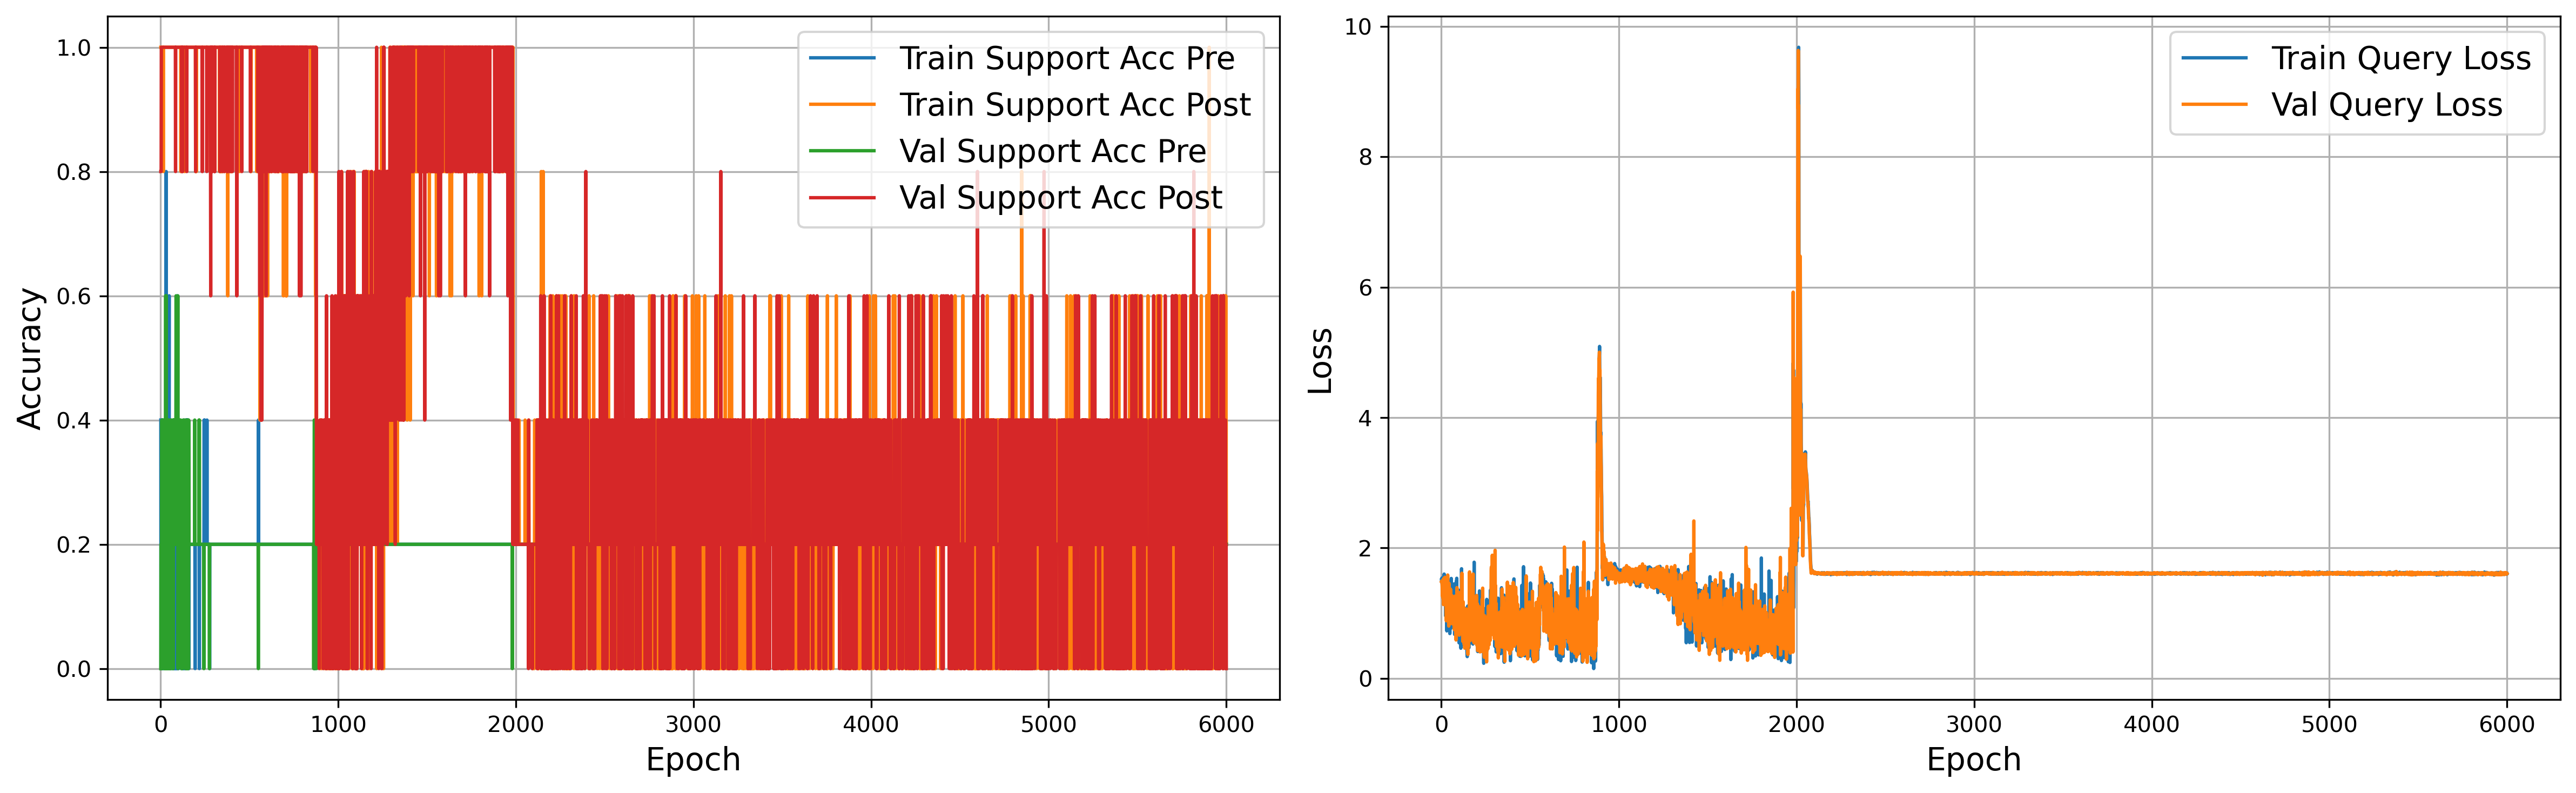
\includegraphics[width=0.8\textwidth]{../images/maml/maml_training.png}
    \caption{Accuracy post adaptación en validación durante el entrenamiento}
    \label{fig:maml training}
\end{figure}

\begin{table}[h!]
\centering

\begin{tabular}{|l|c|c|c|}
\hline
 & Support pre (\%) & Support post (\%) & Query post(\%)\\
\hline
Train & 20 & 100 & 93.33\\
\hline
Validation & 20 & 100 & 92\\
\hline
\end{tabular}
\caption{Accuracies finales de MAML sobre MNIST para support (pre y post) y query (post).}
\label{tab:maml accs}
\end{table}

En la figura~\ref{fig:maml training} se observa la evolución de la accuracy sobre el support set de validación luego de la adaptación interna de MAML. La curva presenta un comportamiento ruidoso, esperable en un entrenamiento episódico con tamaño de meta bache 1. A pesar de estas oscilaciones, la accuracy se mantiene mayormente en valores altos, entre 0.8 y 1.0, lo que indica que el modelo logra ajustarse correctamente a los ejemplos del support set después de los pasos internos de adaptación. Dado que se trabaja en un esquema 5-way 1-shot, el support set contiene solo cinco ejemplos, por lo que la métrica toma valores discretos y puede presentar saltos bruscos entre iteraciones.

La tabla~\ref{tab:maml accs} confirma este comportamiento: antes de la adaptación, la accuracy sobre support es 20$\%$, equivalente al azar en una tarea de cinco clases. Después de la adaptación, la accuracy sobre support alcanza 100$\%$, lo que muestra que el modelo consigue ajustarse perfectamente a los ejemplos disponibles en cada episodio. Sin embargo, la accuracy sobre query después de la adaptación alcanza un valor de 93.33$\%$ en entrenamiento y 92$\%$ en validación, lo que sugiere que el modelo aprende a adaptarse rápidamente a nuevas tareas y generalizar a muestras no vistas.


\subsection{Prototypical Networks, MAML y ProtoMAML}
\begin{figure}[H]
    \centering
    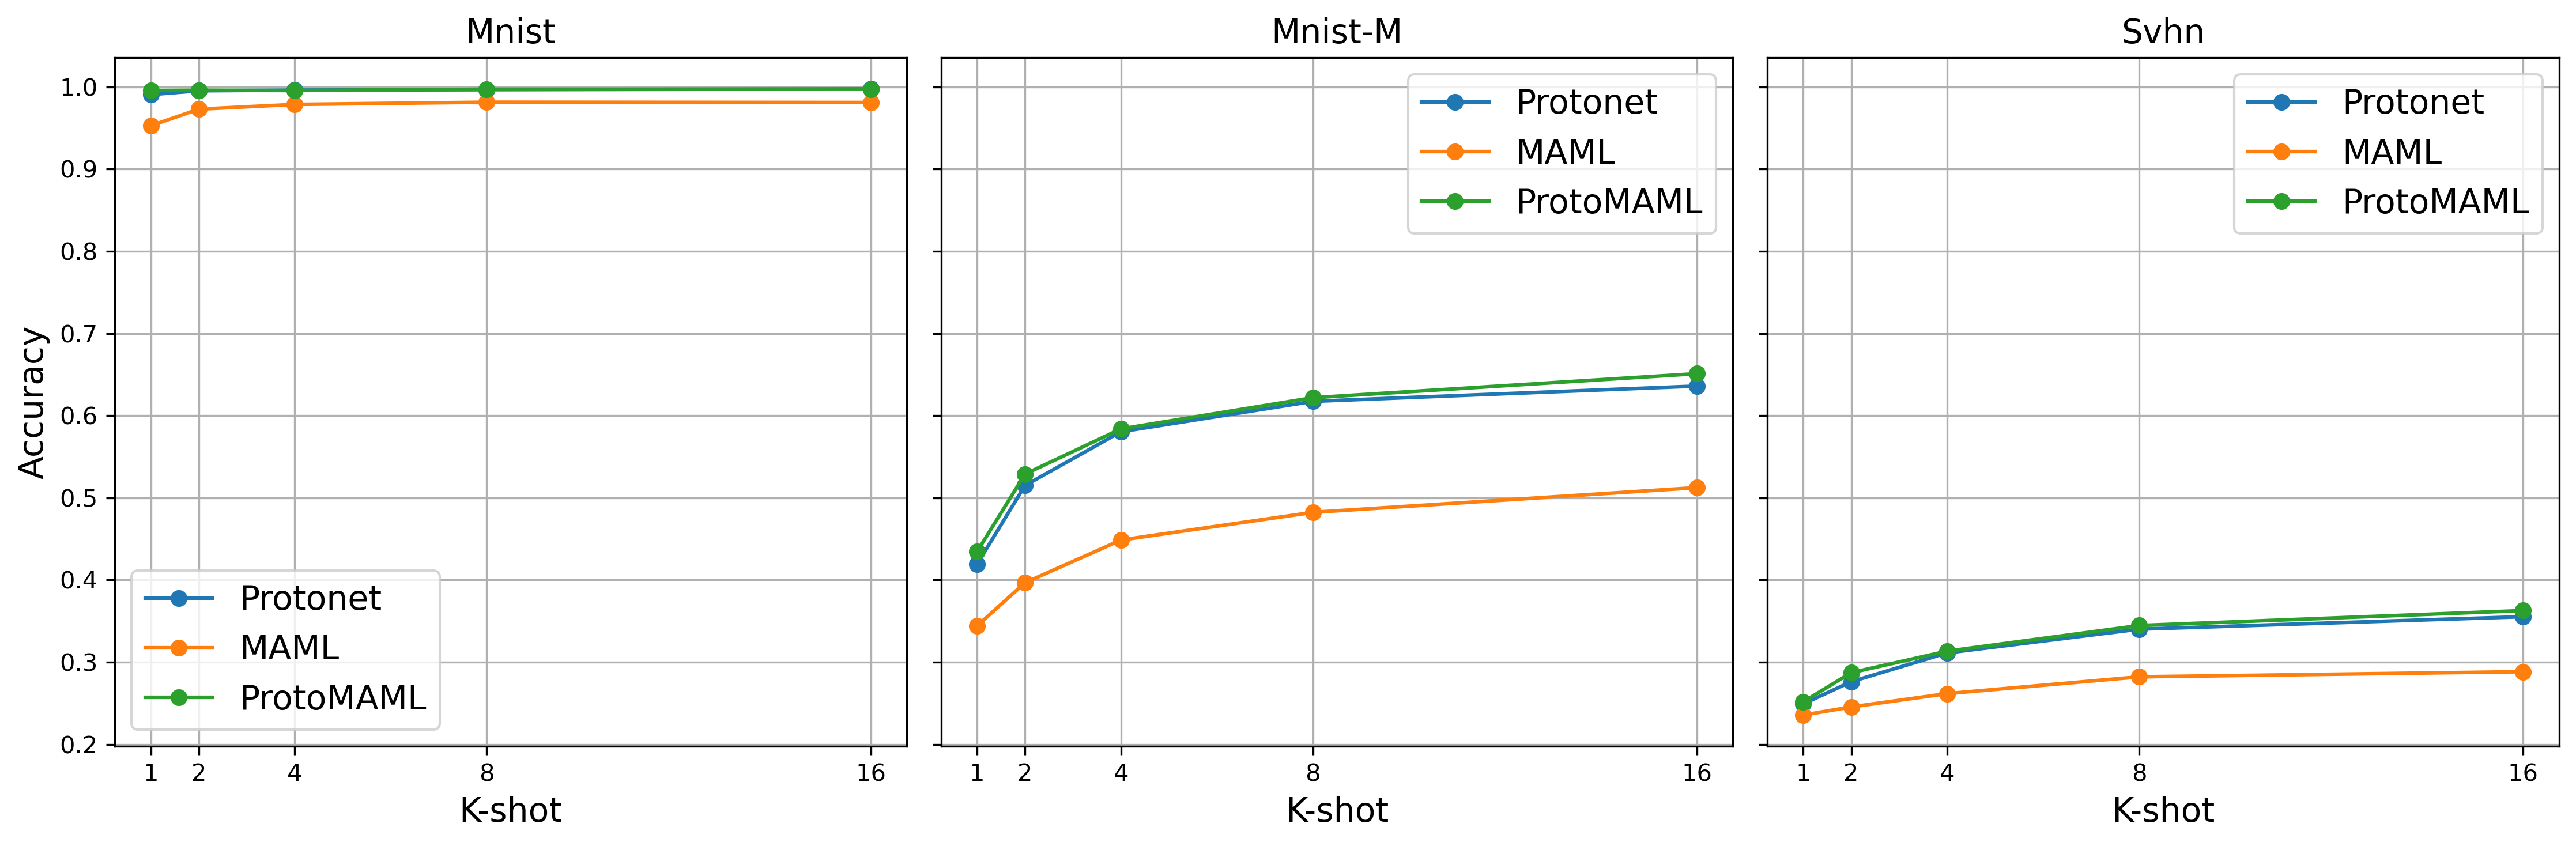
\includegraphics[width=0.9\textwidth]{../images/compare_models/accuracies_ks.png}
    \caption{Accuracy para los tres modelos sobre el conjunto de test de MNIST con k = {1, 2, 4, 8, 16}}
    \label{fig:accuracies ks models}
\end{figure}

En la figura~\ref{fig:accuracies ks models} se comparan ProtoNet, MAML y ProtoMAML para distintos valores de $K$ sobre MNIST, MNIST-M y SVHN. En MNIST, los tres modelos alcanzan accuracies cercanas a 1, lo cual era esperable por tratarse del dominio de entrenamiento. ProtoNet y ProtoMAML se mantienen levemente por encima de MAML.

En los dominios cross-domain, MNIST-M y SVHN, la diferencia entre métodos es más clara. ProtoNet y ProtoMAML obtienen mejores resultados que MAML para todos los valores de $K$, lo que sugiere que los enfoques basados en prototipos son más robustos frente al cambio de dominio.

El resultado destacado de esta figura es que ProtoMAML logra resultados similares o incluso levemente superiores a ProtoNet, aún siendo entrenado con la mitad de iteraciones (10.000 a 20.000) y un menor valor de $K$ (1 a 5). Esto parece indicar que ProtoMAML aprovecha la combinación entre representación prototípica y adaptación interna. MAML, por su parte, queda por debajo, lo que muestra que la adaptación por gradiente con pocos ejemplos no es suficiente para compensar el cambio de dominio.  

\begin{figure}[H]
    \centering
    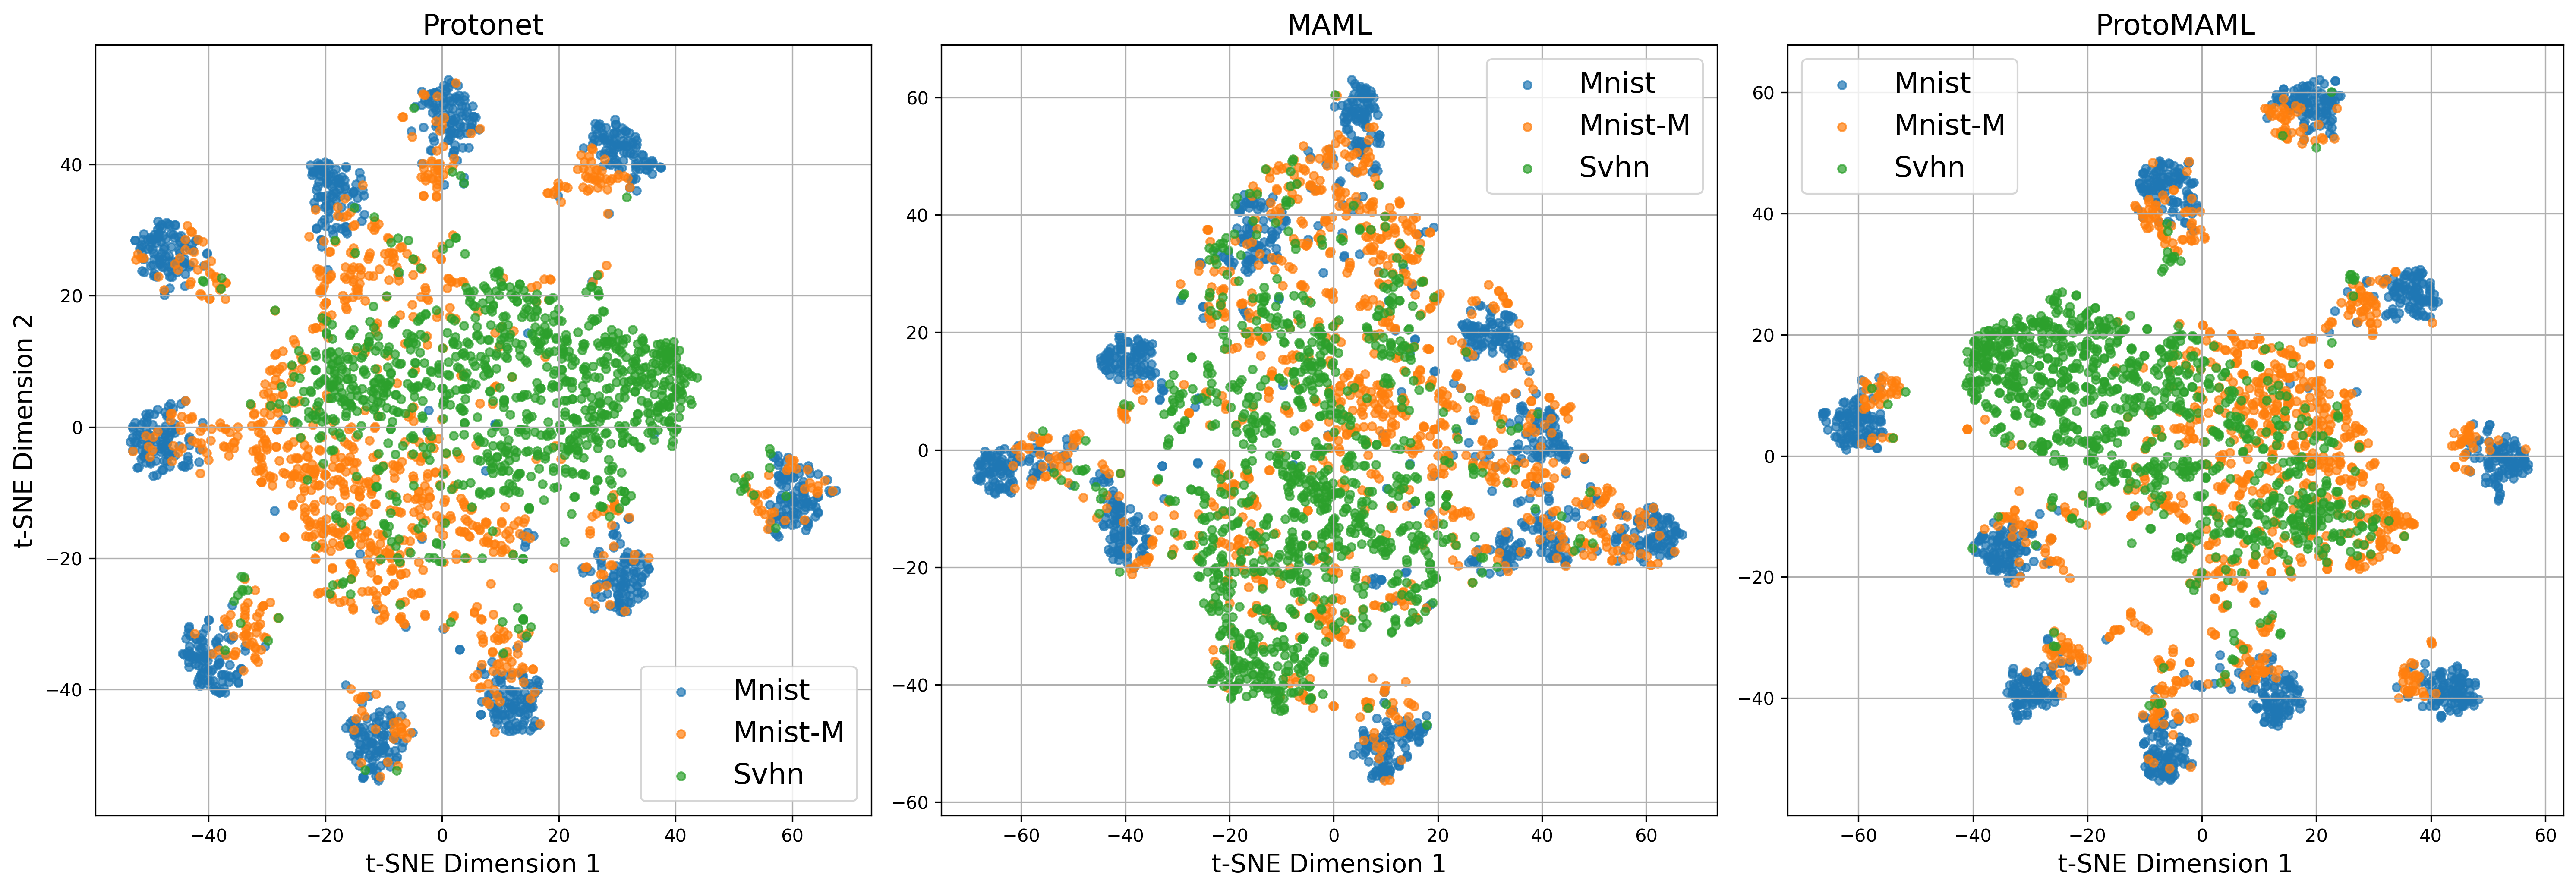
\includegraphics[width=0.8\textwidth]{../images/compare_models/models_tsnes.png}
    \caption{t-SNE de los embeddings de los encoders de los tres modelos para un conjunto de imágene de prueba sobre los tres dominios.}
    \label{fig:models tsnes}
\end{figure}


% Visualización del espacio latente comparativa: proyectar los embeddings del encoder para imágenes de MNIST, MNIST-M y SVHN en el mismo gráfico, usando el encoder de cada modelo. Colorear por dominio. ¿Qué modelo produce embeddings más cercanos entre dominios? ¿Se corresponde con la accuracy cross-domain?

En la figura~\ref{fig:models tsnes} se comparan los embeddings generados por ProtoNet, MAML y ProtoMAML, coloreados según el dominio. Se puede observar que los modelos de Protonet y ProtoMAML muestran una mayor cercanía entre los embeddings de MNIST y MNIST-M, especialmente en algunos grupos de clases donde ambos dominios aparecen parcialmente superpuestos. SVHN, en cambio, permanece más separado y disperso, lo cual coincide con sus menores valores de accuracy. MAML presenta una estructura menos alineada entre dominios, lo que se refleja también en su peor desempeño en cross-domain.


En conjunto, ProtoMAML parece producir los embeddings más cercanos entre dominios, seguido de ProtoNet. Esta observación es consistente con los resultados de accuracy mostrados en la figura~\ref{fig:accuracies ks models}, ya que ambos modelos superan a MAML en MNIST-M y SVHN.

\subsection{DANN}

\begin{figure}[H]
    \centering
    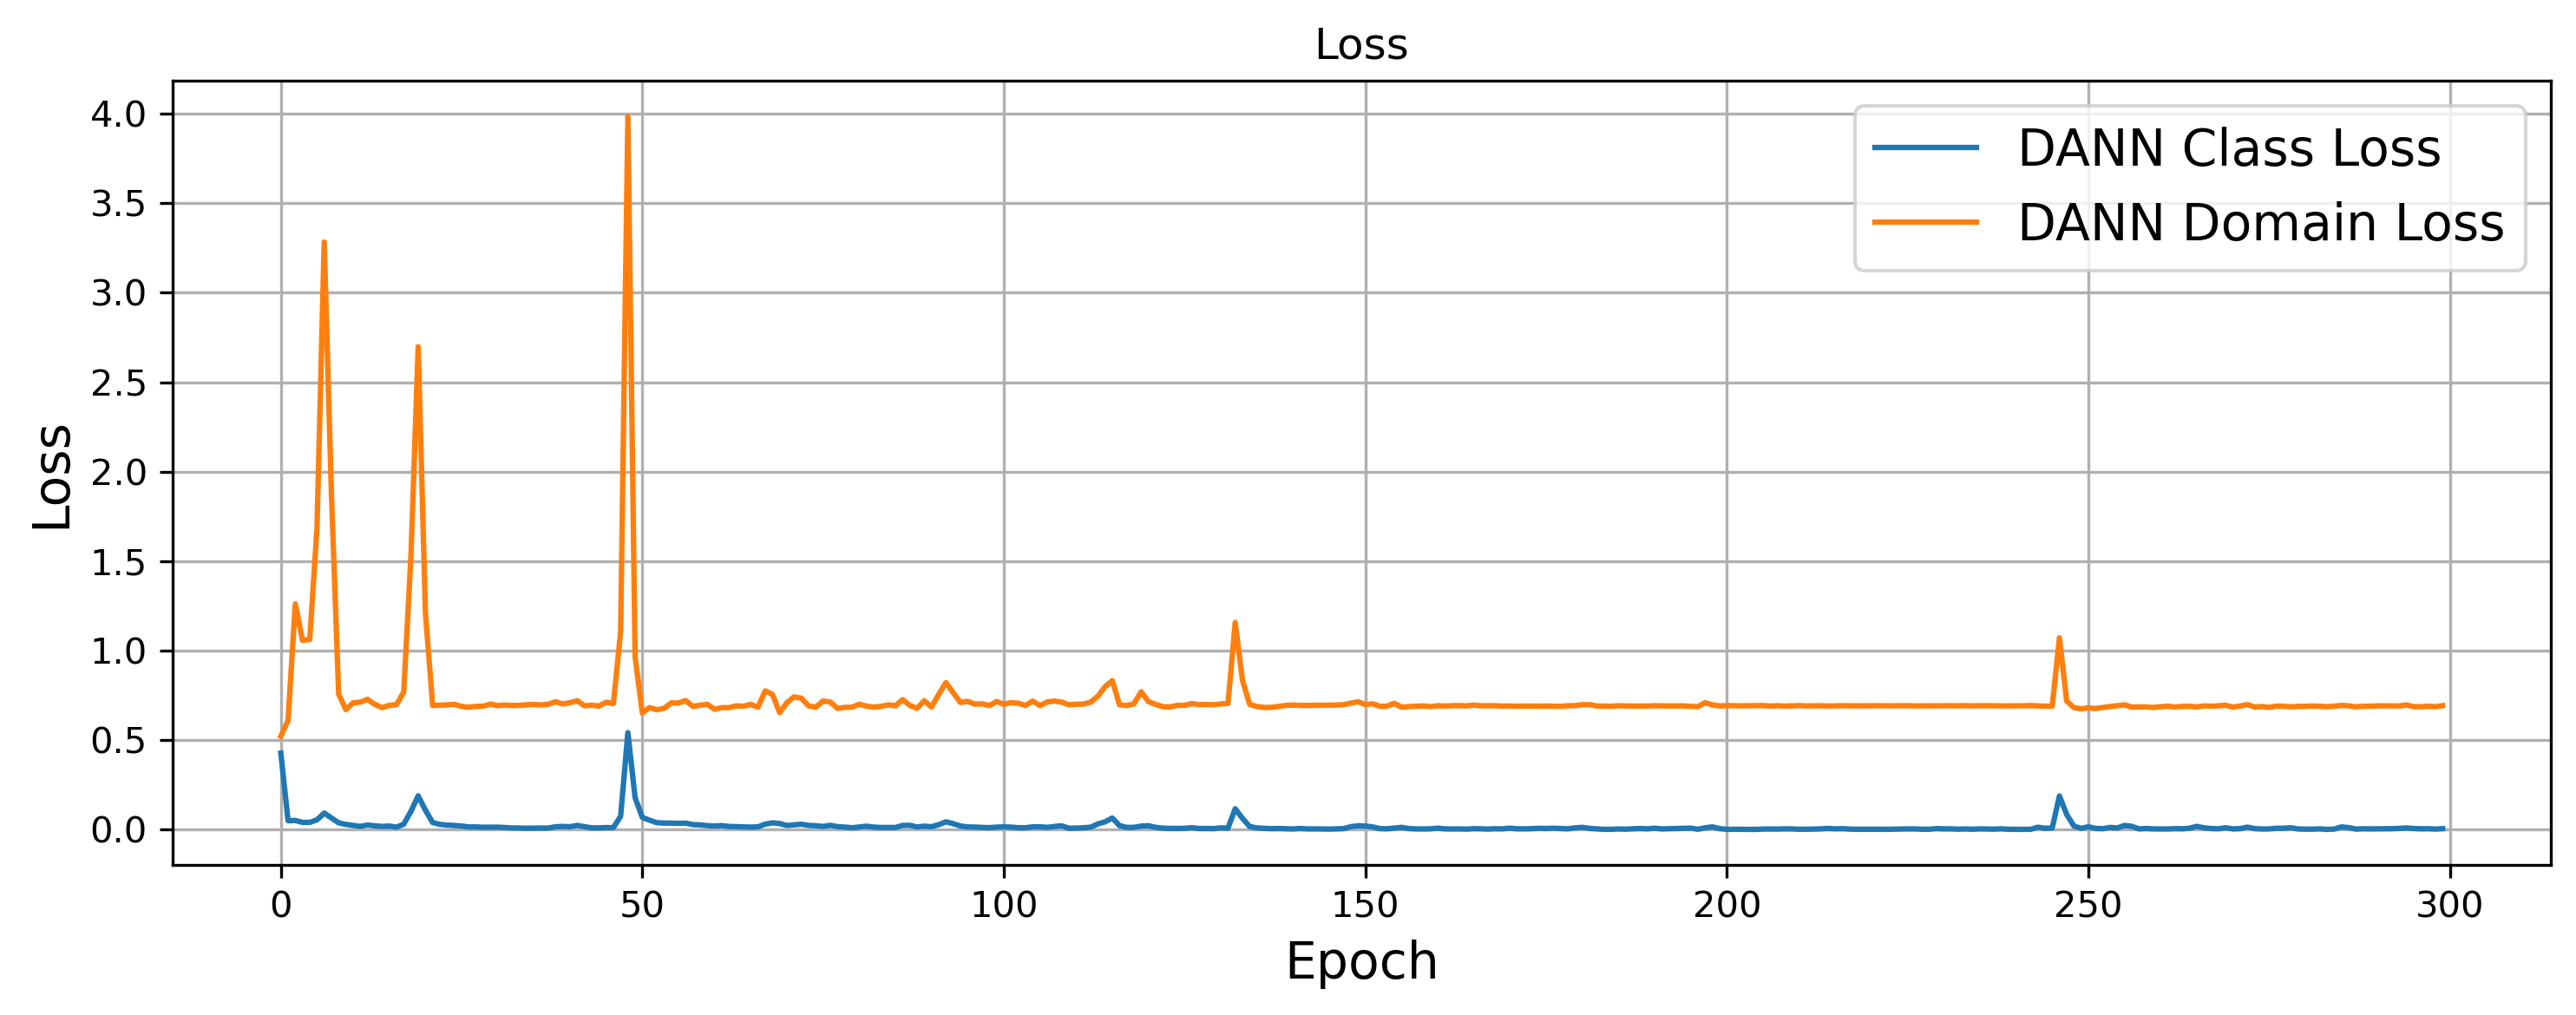
\includegraphics[width=0.8\textwidth]{../images/dann/dann_training_loss.png}
    \caption{Perdida de clasificación y dominio durante el entrenamiento de DANN.}
    \label{fig:dann loss}
\end{figure}

% Graficar en el mismo plot la loss de clasificación, la loss de dominio y la accuracy en MNIST-M a lo largo del entrenamiento, para DANN y el baseline. ¿Cómo evolucionan en relación la una con la otra?

En la figura~\ref{fig:dann loss} se tienen las pérdidas de clasificación y de dominio del modelo DANN durante el entrenamiento. Se observa que ambas tienen oscilaciones correspondientes al tipo de entrenamiento adversarial, presentando picos en epocas similares, pero perdida de dominio los presenta con escalas mayores.

Para comparar el entrenamiento del modelo DANN con el modelo baseline, en la siguiente figura se representa únicamente la pérdida de clasificación. Se omite la pérdida de dominio para facilitar la visualización, ya que su escala es considerablemente mayor y dificulta la comparación.

\begin{figure}[H]
    \centering
    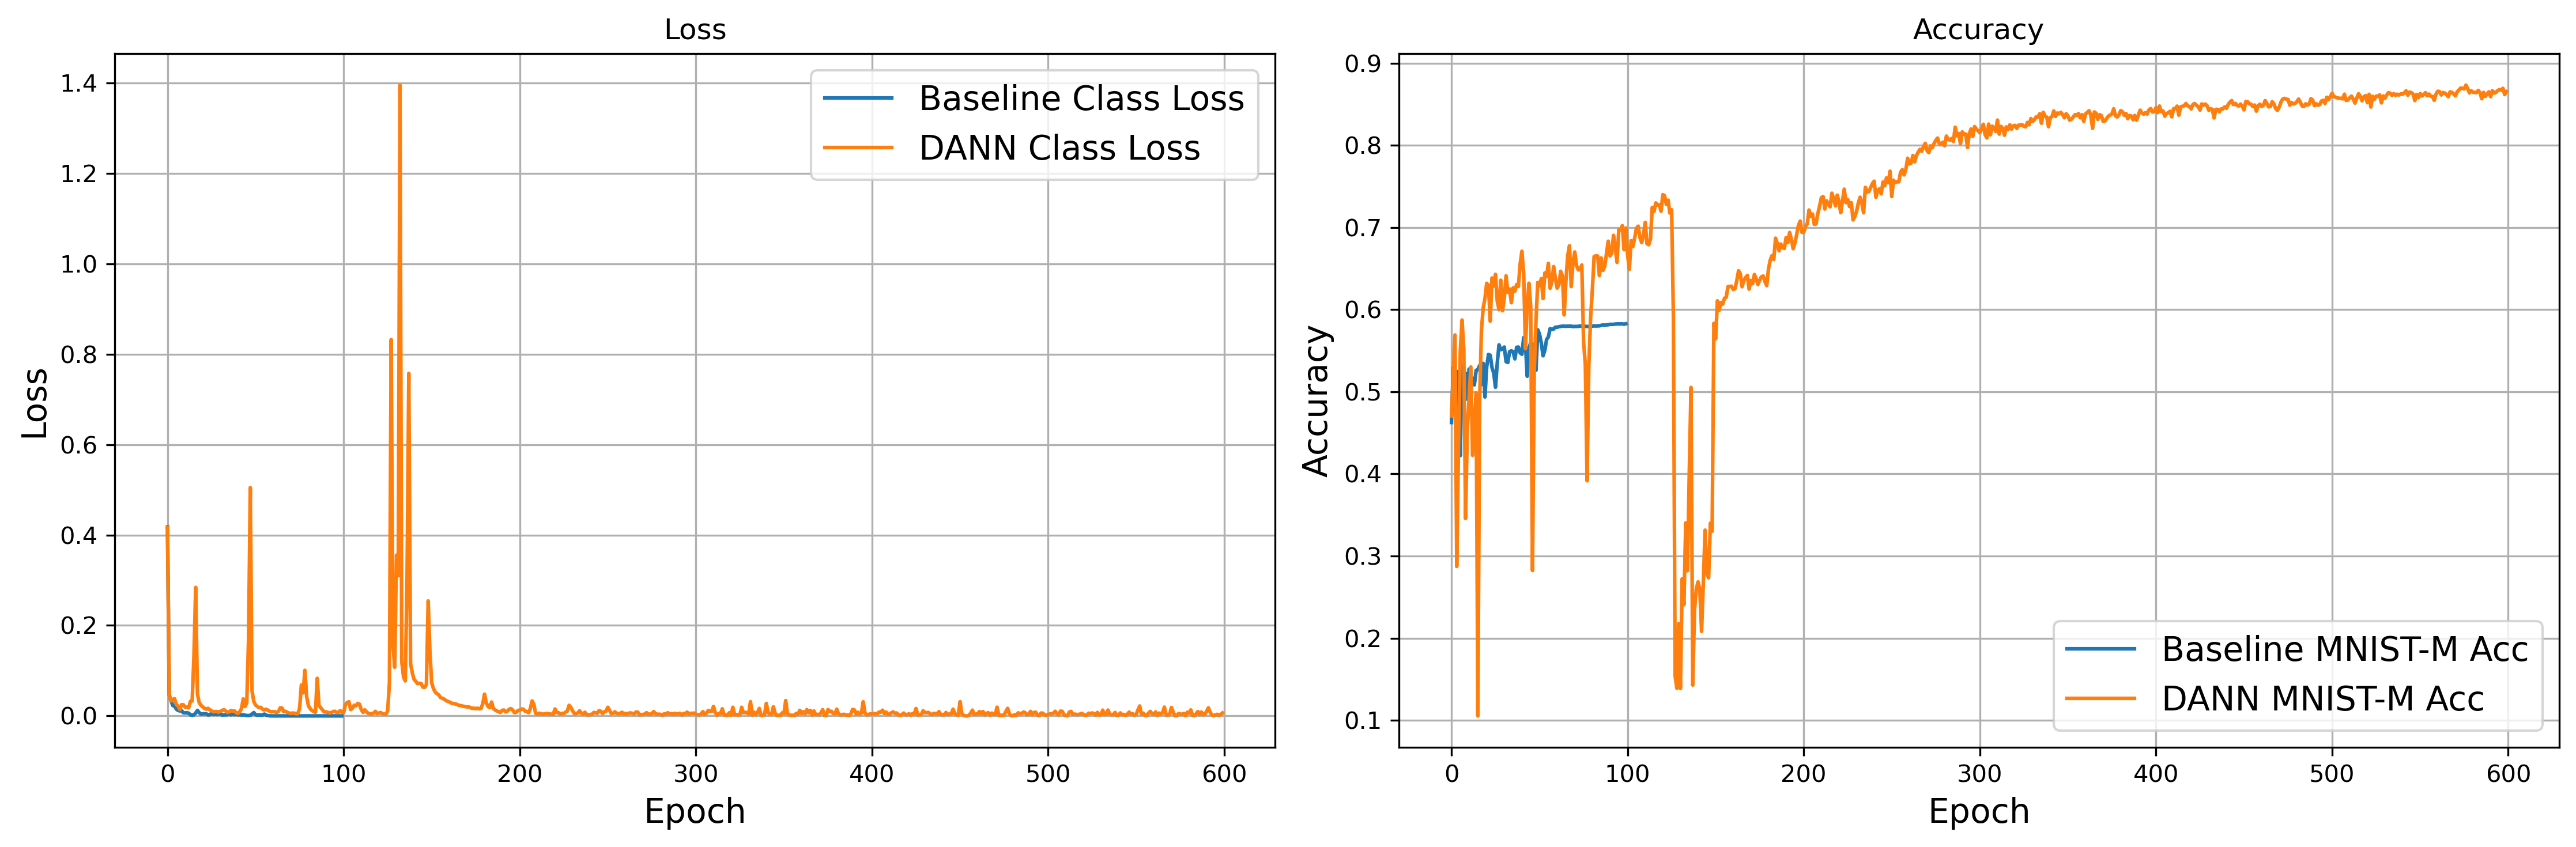
\includegraphics[width=0.8\textwidth]{../images/dann/dann_baseline_training.png}
    \caption{Perdida de clasificación y accuracy durante el entrenamiento del baseline y DANN.}
    \label{fig:dann baseline training}
\end{figure}

En la figura~\ref{fig:dann baseline training} para la loss de clasificación se observa que el baseline converge rápidamente, aproximadamente en la época 25. Sin embargo, a partir de ese punto su accuracy sobre MNIST-M empieza a disminuir levemente, lo que puede significar un sobre ajuste sobre MNIST y una perdida de generalización entre dominios. 

En cambio, DANN presenta un entrenamiento más ruidoso, con picos en la pérdida posiblemente asociados a la dinámica adversarial introducida por el discriminador de dominio y la GRL. A pesar de esa inestabilidad inicial, el modelo logra reducir progresivamente la pérdida y aumentar de manera sostenida la accuracy sobre MNIST-M, alcanzando un desempeño superior al baseline. Esto indica que el entrenamiento adversarial favorece la construcción de representaciones más transferibles entre dominios.

\begin{table}[h!]
\centering

\begin{tabular}{|l|c|c|c|}
\hline
 & MNIST (\%) & MNIST-M (\%)\\
\hline
Baseline & 99.51 & 56.45\\
\hline
DANN & 99.06 & 86.35\\
\hline
\end{tabular}
\caption{Accuracies sobre test de los modelos baseline y DANN para los tres dominios.}
\label{tab:tabla dann}
\end{table}

A partir de la tabla~\ref{tab:tabla dann}, se observa que el baseline obtiene un rendimiento apenas superior en MNIST, con una diferencia de $0.45\%$ respecto de DANN. Sin embargo, en MNIST-M la diferencia se invierte de manera significativa: DANN alcanza una accuracy de $86.35\%$, frente al $56.45\%$ del baseline, una mejora de aproximadamente $30\%$ en el dominio objetivo. Este resultado tiene sentido al considerar que baseline se entrena solamente para clasificar MNIST, mientras que DANN usa parte de su optimización para confundir al discriminador, logrando generalizar a MNIST-M.

\begin{figure}[H]
    \centering
    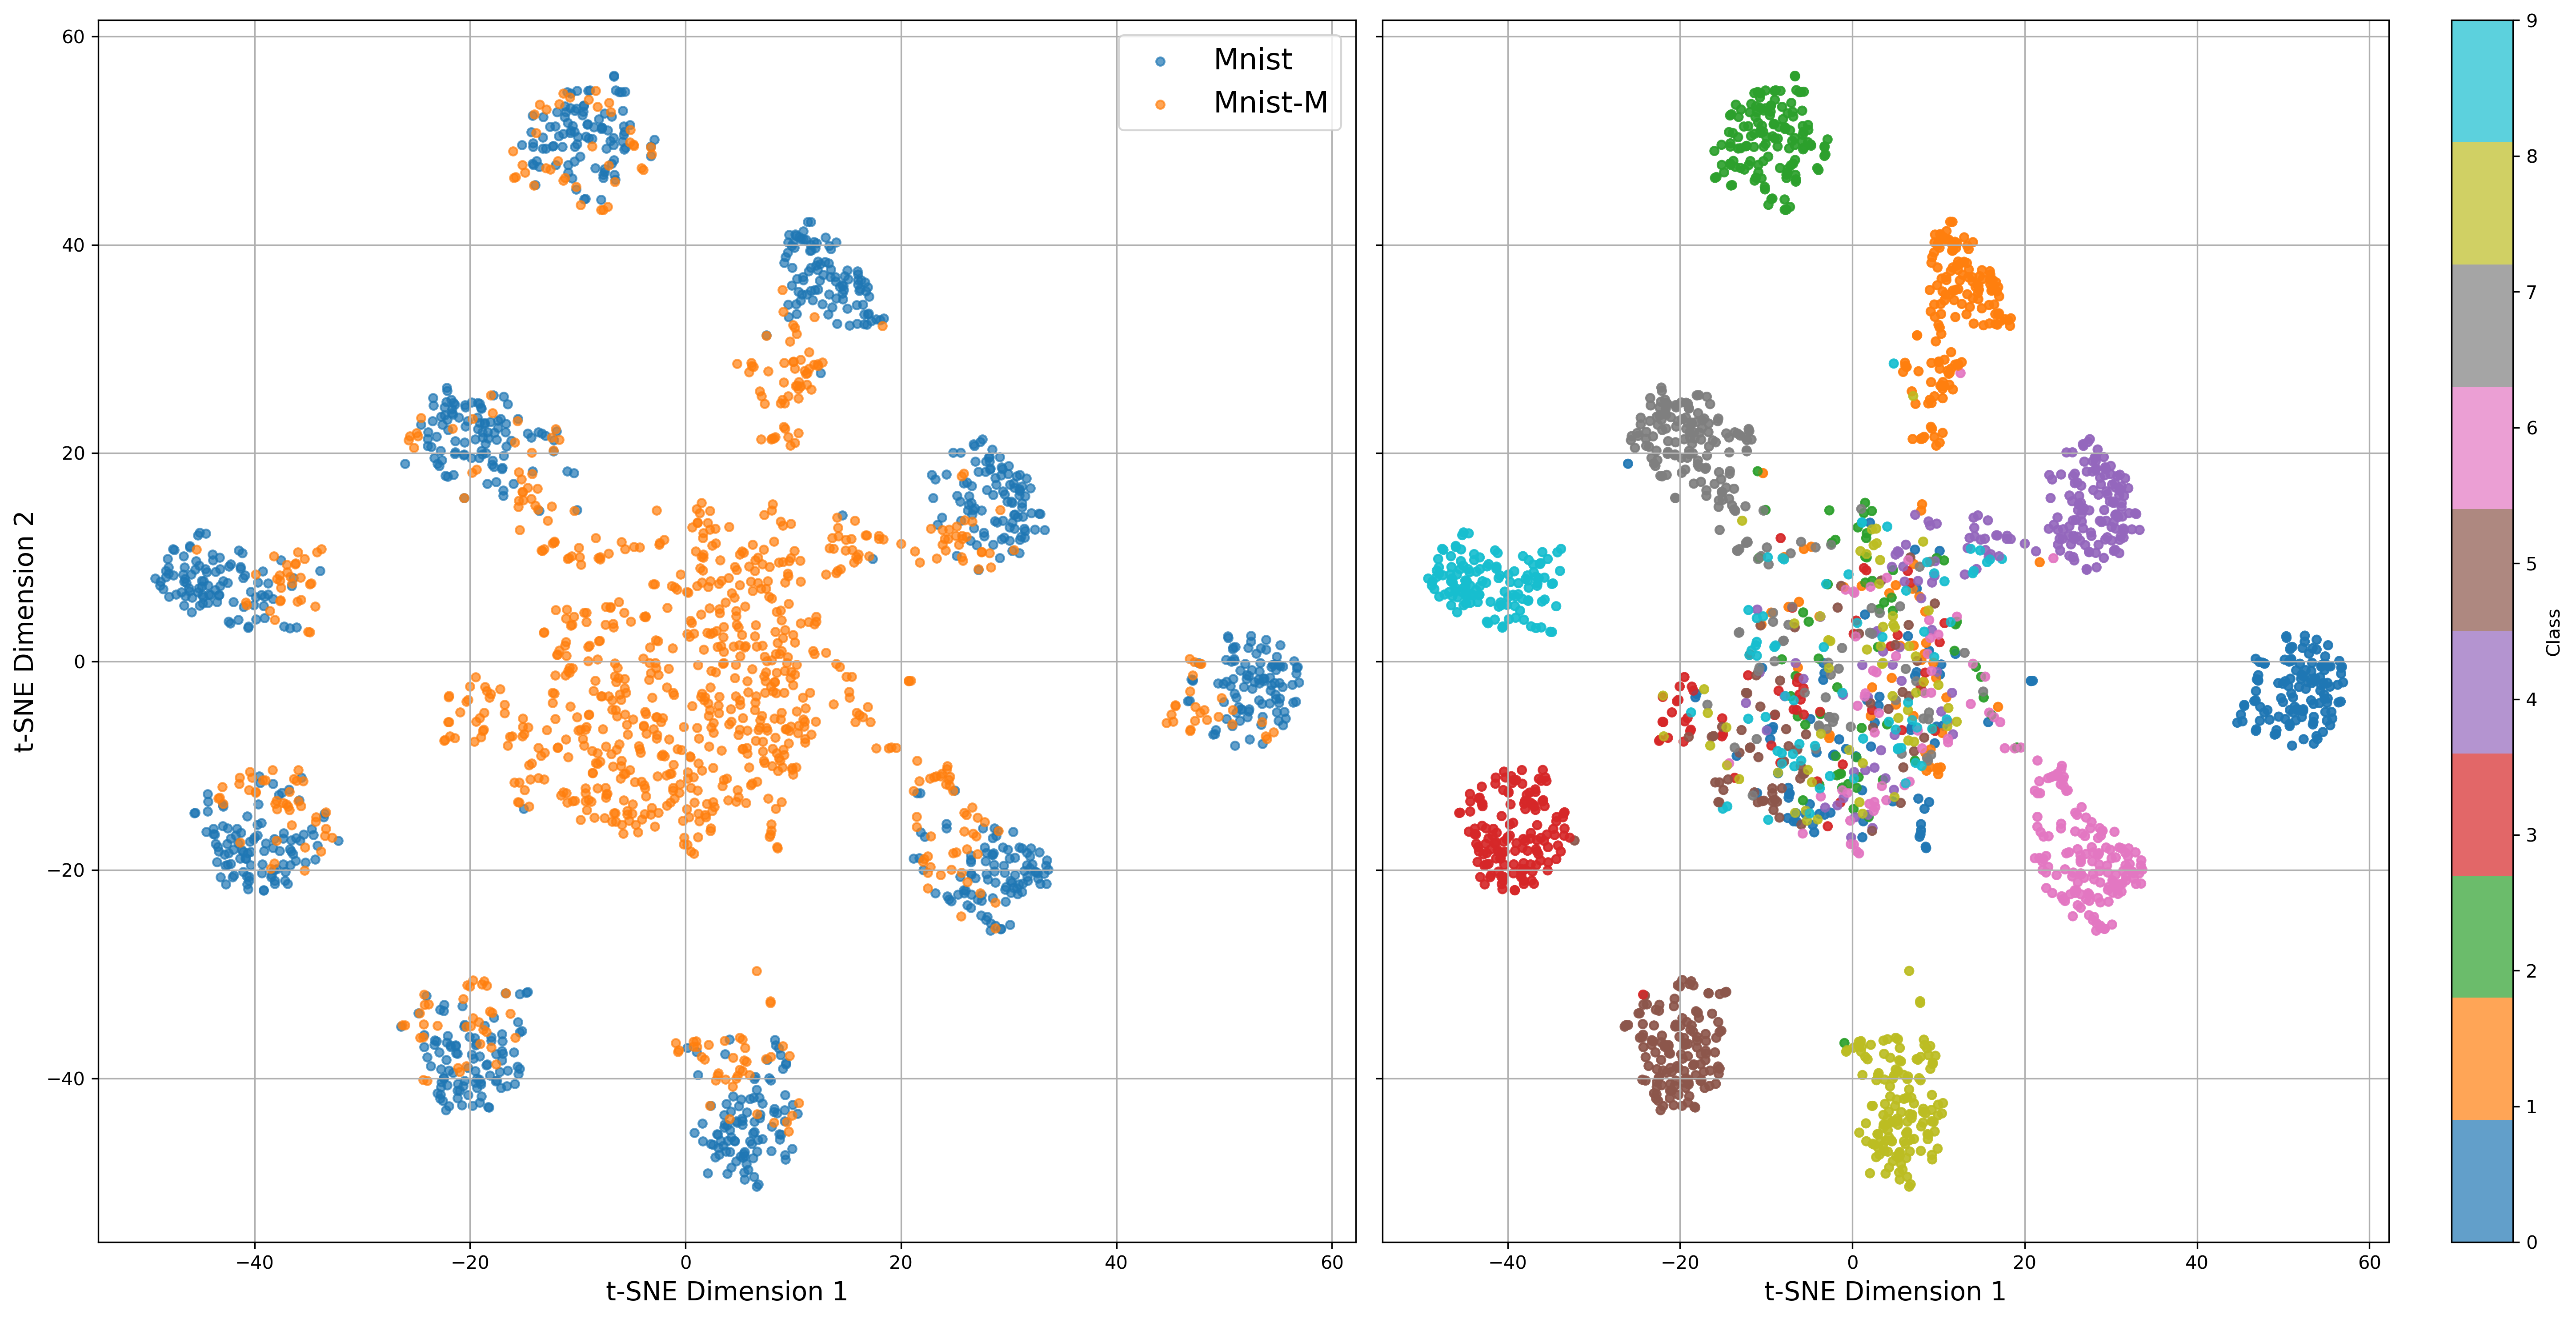
\includegraphics[width=0.8\textwidth]{../images/dann/baseline_tsne.png}
    \caption{t-SNE de los embeddings del encoder del baseline para un conjunto de imágene de prueba sobre MNIST y MNIST-M.}
    \label{fig:baseline tsne}
\end{figure}


\begin{figure}[H]
    \centering
    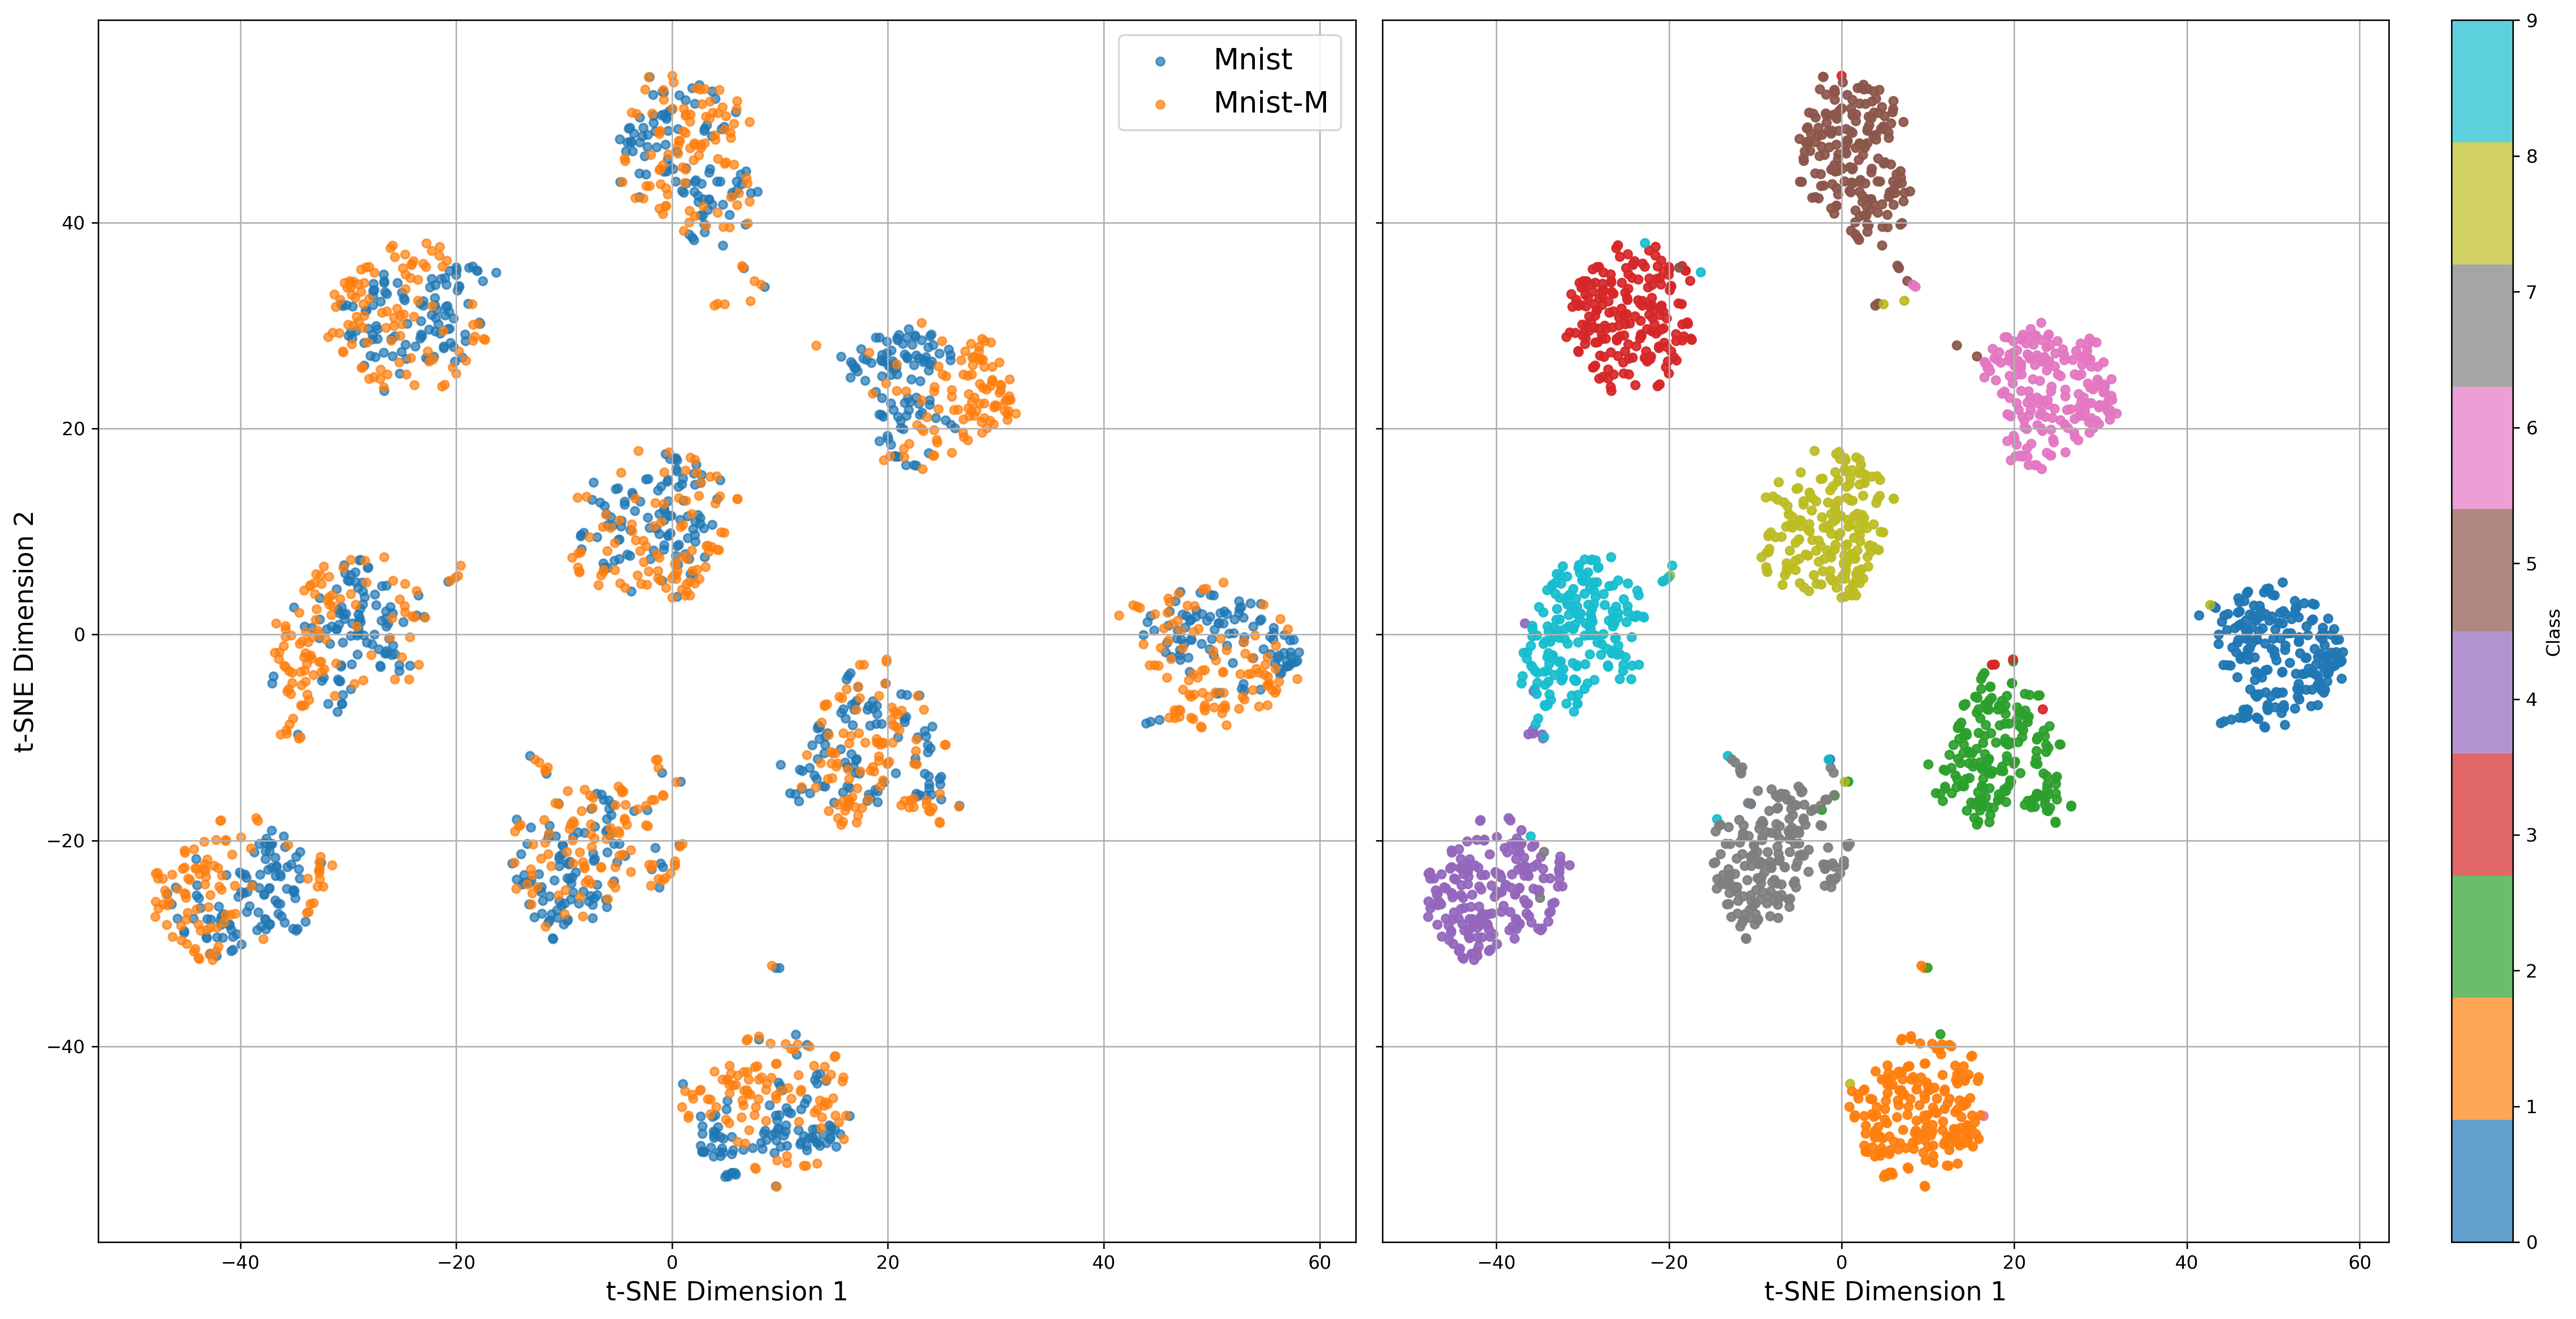
\includegraphics[width=0.8\textwidth]{../images/dann/baseline_ft_tsne.png}
    \caption{t-SNE de los embeddings del encoder del baseline finetuned para un conjunto de imágene de prueba sobre MNIST y MNIST-M.}
    \label{fig:baseline ft tsne}
\end{figure}


\begin{figure}[H]
    \centering
    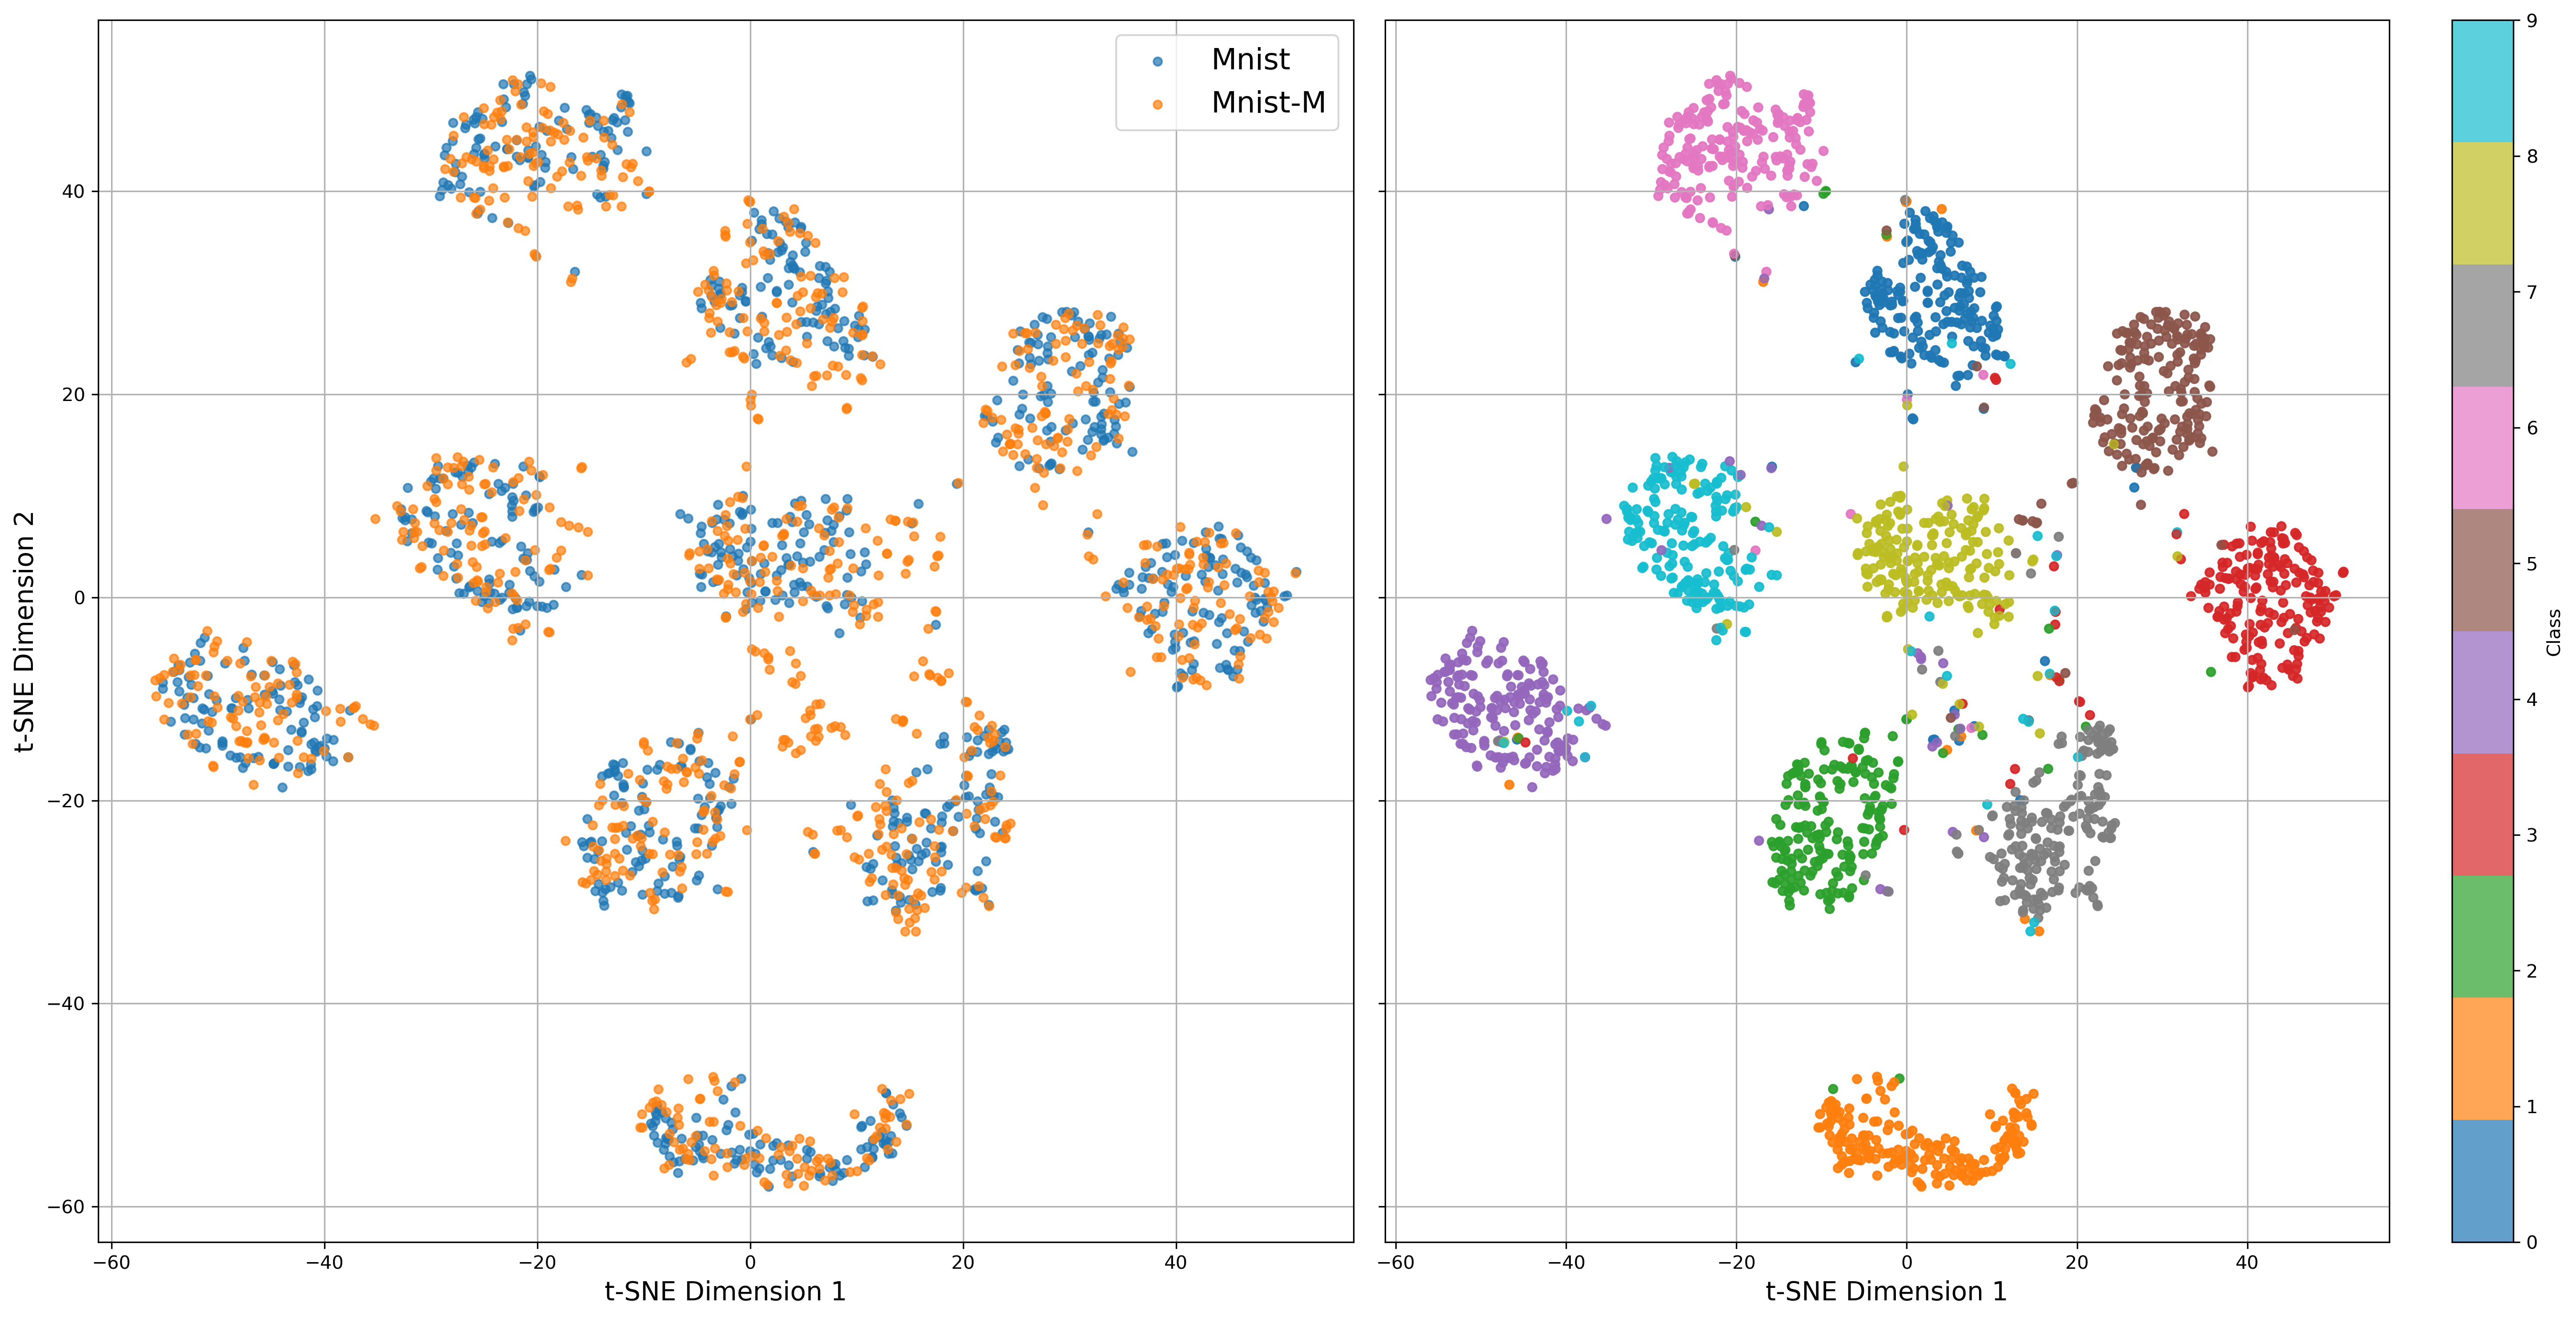
\includegraphics[width=0.8\textwidth]{../images/dann/dann_tsne.png}
    \caption{t-SNE de los embeddings del encoder de DANN para un conjunto de imágene de prueba sobre MNIST y MNIST-M.}
    \label{fig:dann tsne}
\end{figure}

A partir de las figuras~\ref{fig:baseline tsne},~\ref{fig:baseline ft tsne} y~\ref{fig:dann tsne}, se observa que el baseline es el modelo que presenta la peor organización del espacio latente. Si bien algunas clases de MNIST aparecen agrupadas, las muestras de MNIST-M quedan más dispersas y se concentran en una zona central con mayor mezcla entre clases.

Luego del fine-tuning, la separación por clase mejora de manera considerable: los clusters se vuelven más definidos y disminuye la mezcla entre muestras de distintas clases. Este resultado es esperable, ya que este modelo es el \textit{upper bound}.

Por su parte, DANN también muestra una mejora clara respecto del baseline. Los embeddings de MNIST y MNIST-M aparecen más alineados dentro de varios clusters, lo que sugiere que el entrenamiento adversarial favorece representaciones más invariantes al dominio. Aunque el baseline con fine-tuning logra una separación visual más limpia, DANN obtiene esta mejora mediante adaptación adversarial, sin depender de un ajuste supervisado sobre el dominio objetivo.  